\documentclass[12pt,a4paper]{report}
\usepackage[utf8]{inputenc}
\usepackage{amsmath}
\usepackage{amsfonts}
\usepackage{amssymb}
\usepackage{amsthm}
\usepackage{natbib}
\usepackage{titlesec}
\usepackage{tikz}
\usepackage{setspace}
\usepackage{hyperref}
\usepackage{frontespizio} 
\usepackage[mathscr]{euscript}
\usepackage[a4paper,left=3.5cm,right=2.5cm]{geometry}
\usepackage[ruled,linesnumbered]{algorithm2e}
\SetKw{KwBy}{by}

\setcounter{secnumdepth}{4}
\setcounter{tocdepth}{4}

\onehalfspacing

% Custom commands...
\newcommand{\Cross}{\mathbin{\tikz [x=2.5ex,y=2.5ex,line width=.10ex] \draw (0,0) -- (1,1) (0,1) -- (1,0);}}
\newcommand{\mathDef}{\overset{\textit{def}}{=}}
\newcommand{\N}{\mathbb{N}}
\newcommand{\R}{\mathbb{R}}
\newcommand{\Rplus}{\mathbb{R}^+}
\newcommand{\SetMinusZero}{\setminus \left\{0\right\}}
\newcommand{\SetFromOneTo}[1]{\N \cap \left[1,#1\right]}
\newcommand{\ItalicQuotMark}[1]{``\textit{#1}"}


\hypersetup{
    colorlinks=true, %set true if you want colored links
    linktoc=all,     %set to all if you want both sections and subsections linked
    linkcolor=black,  %choose some color if you want links to stand out
}


\begin{document}
	
\begin{frontespizio} 
	\Universita{Roma ``Tor Vergata'' } 
	\Logo[3cm]{./images/logo}
	\Facolta{Ingegneria} 
	\Corso[Laurea Magistrale]{Ingegneria Informatica} 
	\Annoaccademico{2020--2021} 
	\Titolo{??}
	\NCandidato{Studente} 
	\Candidato[0273395]{Andrea Graziani} 
	\NRelatore{Docente}{} 
	\Relatore{Prof.ssa Valeria Cardellini}
	\Correlatore{Dott. Gabriele Russo Russo}
\end{frontespizio} 
	
	
\tableofcontents

\chapter{Introduction}

\section{The Serverless Computing Paradigm}

In recent years, thanks to an increased popularity of several lightweight virtualization solutions, specifically containers and container-orchestration systems, many public cloud providers have launched a new set of cloud computing services belonging to new service's type category called \textit{Function-as-a-Service} (\textit{FaaS}), where almost every aspect of the system administration tasks needed to deploy a workload on the cloud, like provisioning, monitoring, resource management and scaling, are directly managed by the provider with a minimum involvement of the user.

With the development of FaaS platforms, the \textit{serverless computing paradigm}, a new application service model according to which any application is abstracted as a group of functions hosted on FaaS platforms orchestrated in a workflow, has emerged. 

Regarding cloud application development, serverless computing paradigm provides many advantages, among which:

\begin{itemize}
	
	\item the providing of a new simplified programming model which helps  developers to focus on logic and business aspects of their applications only, without worry about the managing of servers. 
	
	This can lead to a development cost reduction decreasing go-to-market time of the software products.
	
	\item the adopting of a very small-granularity billing pricing model called “\textit{pay as you go}”, by charging for execution time rather than for allocated resources. which can decrease the cost substantially.
	
	The small-granularity billing and scaling in
	FaaS platforms can also decrease the cost substantially
	
	
	
	
	\item Moreover, the paradigm lowers the cost of deploying applications too, adopting a so-called “\textit{pay as you go}” pricing model, by charging for execution time rather than for allocated resources \cite{COSE}.
\end{itemize}

 





In serverless computing platforms, computation is done by so-called \textit{function instances} which are completely managed by the serverless computing platform provider and act as tiny servers that can be invoked based on events forwarded by end-users \cite{PMSCP}.





\subsection{Serverless Function}

A \textit{serverless function} represents a stateless, event-driven, self-contained unit of computation implementing a business functionality.

Although a serverless function generally represents a unit of executable code, submitted to FaaS platforms by developers using one or a combination of the programming languages supported by FaaS providers, a serverless function can be any cloud services eventually necessary to business logic, like cloud storage, message queue services, pub/sub messaging service etc.

When it represents executable code, developers can specify several configuration parameters, like timeout, memory size or CPU power \cite{COSE}.

A serverless function can be triggered through events or HTTP requests following which the FaaS provider executes it in a containerized environment, like container, virtual machine or even processes, using the specified configuration.

\subsection{Serverless Application}

In serverless paradigm, the most basic scenario is to invoke a single function through a HTTP request; however, if you want to built more complex applications, constructing so-called \textit{serverless application}, serverless functions must be connected and appropriately coordinated.

Formally, we define a serverless application as a stateless and event-driven software system made up of a serverless functions set hosted on one or more FaaS platforms and combined together by a so-called \textit{coordinator} (or \textit{orchestrator}).

Generally, the coordinator is a broker needed to implement the business logic of any application: it chains together serverless function, handles events among functions and triggers them in the correct order according to the business logic defined by developers. 

Most public cloud providers for serverless computing have introduced platforms to define and coordinate serverless function in order to built serverless application, like AWS Step Functions which combines multiple Lambda functions and other serverless services offered by AWS into responsive serverless applications

Although FaaS platforms continuously advance the support for serverless applications, existing solutions are dominated by a few large-scale providers resulting in mostly non-portable FaaS solutions 

and provider lock-in

occurs when transitioning data, products, or services to another vendor's platform is difficult and costly, making customers more dependent (locked-in) on a single cloud storage solution.

FC languages and runtime systems are still in their
infancy with numerous drawbacks. Current commercial and open
source offerings of FC systems are dominated by a few large-
scale providers who offer their own platforms, 

As FaaS platforms take over operational responsibilities,
besides uploading the source code of functions, users have
limited control over resources on FaaS platforms. Taking
AWS Lambda as an example, the amount of allocated mem-
ory during execution and the concurrency level are only op-
tions for tuning the performance of functions. The amount
of allocated memory is between 128 MB and 3,008 MB
in 64MB increments [13]. Previous researches have proven
that computational power and network throughput are in
proportion to the amount of allocated memory, and disk
performance also increases with larger memory size due
to less contention [14], [15]. By reserving and provisioning
more instances to host functions, high concurrency level can
decrease fluctuations in the function performance incurred
by cold starts (container initialization provisioning delay if
no warm instance is available) and reduce the number of
throttles under very heavy request loads



\subsection{fdsfsd}




\begin{itemize}
	\item 
\end{itemize}

\subsection{title}





the run-time of these serverless
functions decreases with the increase of memory size allocated
to the function. However, the marginal improvement in the
run-time decreases as the memory increases.

This behavior
is because the pricing model as exposed by the cloud providers
is tightly coupled with the amount of resources specified
to execute the serverless function (c.f. Figure 1a), and the
dependency between memory and CPU resource allocation –
AWS Lambda allocates CPU power


a model for each executable belonging to a given choreography.



This helps developers decide if a developed
workload would comply with their QoS agreements, and if
not, how much performance improvement they would need
to do so. The performance improvement decided could be
achieved either by improving the design, quality of code, or
by simply resizing the resource allocated to each instance,
which is usually set by changing the allocated memory.


A cold start 

Cold/Warm start: as defined in previous work [3], [8],
[10], we refer to cold start request when the request goes
through the process of launching a new function instance.
For the platform, this could include launching a new virtual
machine, deploying a new function, or creating a new
instance on an existing virtual machine, which introduces an
overhead to the response time experienced by users. In case
the platform has an instance in the idle state when a new
request arrives, it will reuse the existing function instance
instead of spinning up a new one. This is commonly known
as a warm start request. Cold starts could be orders of
magnitude longer than warm starts for some applications.
Thus, too many cold starts could impact the application’s
responsiveness and user experience [3].



his equation gives the probability of a request being
rejected (blocked) by the warm pool, assuming there are m
warm servers. If m is less than the maximum concurrency
level, the request blocked by the warm pool causes a cold
start. If the warm pool has reached the maximum concur-
rency level, any request rejected by the warm pool will be
rejected by the platform.


\section{Motivations}

Although serverless computing paradigm makes cloud application developing easier guaranteeing a cost-effective solution, there are several obstacles that prevent FaaS platforms to support more general workloads.

Scientific literature have already reported a huge amount of limitations preventing a worldwide adoption, among which we recall:

\begin{itemize}
	
	\item the lack of support for those applications having fine-grained state sharing needs, which is primarily due to stateless nature of serverless platforms.
	
	\item the absence of fine-grained coordination capabilities between serverless functions.
	
	\item very unpredictable performance due  is the variability in the hardware resources that
	results from giving the cloud provider flexibility to choose the underlying server. 
	
	

\end{itemize}


The examples above highlights some factors that can affect
the performance of running serverless functions. However,
they are not the only factors. A recent study [9] showed
that the underlying infrastructure and resource provisioning
can vary significantly depending on multiple factors including
function placement, cold starts, I/O and network conditions,
type of VMs/containers, and co-location with other functions.


Obliviously, the user cannot control  no control 

is oblivious to all these other factors, and has only
limited control over a few parameters affecting performance,
i.e. memory and processing power.


, especially those that must meet strict guarantees.



First of all, when cloud application developers want to run a serverless function, is necessary to specify several configuration's parameters regarding its execution environment, like RAM memory size, time limits or CPU power; unfortunately configuring such parameters correctly, meeting cost and response time constraints, is not trivial. 

In fact, several studies have already shown that aforementioned configuration parameters significantly affect the cost and response time of any serverless functions. 

\ref{COSE} have shown that serverless function's response time decreases when the RAM memory size, allocated to the function, is increased; however, due to pricing models adopted by the vast majority of FaaS providers, according to which cost depends proportionally on the amount of RAM memory size allocated to a serverless function, a too large value for memory can result in higher costs.

Nevertheless, serverless function's configuration parameters problem is quite more complicated than that, because, due to the tight coupling between the pricing model and the amount of allocated resources, even setting a small value of RAM memory size can lead to higher costs, due to a longer execution time of the functions. Moreover, the marginal improvement in response time decreases as the memory increases.


\subsection{dsadasdasda}

is used, owing to a longer duration, it can lead to higher costs.  




despite a too large a value for memory can result in higher costs for running the function




run-time of these serverless
functions decreases with the increase of memory size allocated
to the function.




FaaS platforms generally exhibit variable performance which precludes their use in applications that must meet strict guarantees.



In fact, despite almost all infrastructure issue are managed by FaaS provider,

Despite there are several factors that can significantly affect the cost and response time of serverless functions, one of the most important is the configuration parameters

Several 
We ran this
function for different memory sizes and studied the effect of
varying memory sizes on the performance of the function, i.e.
run-time. Figure 1b shows how the run-time of these serverless
functions decreases with the increase of memory size allocated
to the function. However, the marginal improvement in the
run-time decreases as the memory increases.



any FaaS provider  requires users to configure
multiple parameters, such as memory, CPU



pricing model as exposed by the cloud providers
is tightly coupled with the amount of resources specified
to execute the serverless function 




Running serverless functions requires users to configure
multiple parameters, such as memory, CPU, cloud provider, etc.
While relatively simpler, configuring such parameters correctly
while minimizing cost and meeting delay constraints is not
trivial. 




Several previous works, have state We ran this
function for different memory sizes and studied the effect of
varying memory sizes on the performance of the function, i.e.
run-time. Figure 1b shows how the run-time of these serverless
functions decreases with the increase of memory size allocated
to the function. However, the marginal improvement in the
run-time decreases as the memory increases. 







Serveless provder performance depend on paramenter that 



In order to meet both functional requirements, concerning the overall logic to be implemented, and non-functional requirements, concerning the quality of service (QoS) levels that should be guaranteed, a system, able to dynamically 

 Such
systems should be able to dynamically adapt themselves
to their environment with little or no human inter-
vention, in order to meet both functional requirements
concerning the overall logic to be implemented and non-
functional requirements concerning the quality of service
(QoS) levels that should be guaranteed.




Serverless computing has given a much-needed agility to
developers, abstracted away the management and maintenance
of physical resources, and provided them with a relatively
small set of configuration parameters: memory and CPU.
While relatively simpler, configuring the “best” values for
these parameters while minimizing cost and meeting perfor-
mance and delay constraints poses a new set of challenges.
This is due to several factors that can significantly affect the
running time of serverless functions.




guarantees both a cost-effective solution and make developing services easier, giving to, FaaS platform generally exhibit variable performance which precludes their use in applications that must meet strict guarantees.
 
 
 Serverless computing is poised to
 make developing services easier, but
 providing QoS guarantees remains
 difficult. 17,27 While the serverless plat-
 form needs to offer some guarantees
 of scalability, performance, and avail-
 ability, this is of little use if the ap-
 plication relies on an ecosystem of
 services, such as identity providers,
 messaging queues, and data persis-
 tence, which are outside the control
 of the serverless platform.
 
 
 
 
 
\begin{enumerate}
	\item scheduling policies today typically imple-
	ment basic rst-come-rst-served algorithms
\end{enumerate}




FaaS and BaaS can exhibit variable
performance which precludes their
use in applications that must meet
strict guarantees.



Despite the fact that serverless solution is cost-effective
and eases the resource management, there are pain points
hindering its wide adoption by potential users, including
the lack of performance and cost model [6], [7], [8], and
the trade-off analysis between the performance and cost
of serverless applications [8], [9]. Performance and cost
modeling and optimization are non-trivial and necessary
steps towards guaranteeing the service level agreement
(SLA) of serverless applications in an economic manner,
which is basically finding an acceptable trade-off between
performance and cost. The difficulties of such modeling and
optimization problems lie in the following aspects:



Serverless computing has given a much-needed agility to
developers, abstracted away the management and maintenance
of physical resources, and provided them with a relatively
small set of configuration parameters: memory and CPU.
While relatively simpler, configuring the “best” values for
these parameters while minimizing cost and meeting perfor-
mance and delay constraints poses a new set of challenges.
This is due to several factors that can significantly affect the
running time of serverless functions.



While many FaaS oerings exist [3, 4, 10, 12, 15, 17, 18, 20],
relatively basic techniques to manage serverless function
invocations are provided today. As function requests are re-
ceived, the cloud provider schedules functions, mostly in
a rst-in-rst-out manner. 


Opportunities to invoke a more
informed scheduling policy are missed, however, in chal-
lenging scenarios such as when incoming demands cannot
be satised by currently available resources. Such scenarios
occur when providers cannot accommodate a rise of invo-
cations due to cold starts or inecient resource allocation
or alternatively when function invocation limits are imposed.
Function invocation limits bound the number of functions
running either instantaneously or over a time period. Be-
cause serverless technologies automatically scale to meet
demands, function invocation limits ensure a bug or miscon-
guration in tenant workloads does not inappropriately scale.
In addition, limits help developers manage costs and better


Thus, a prospective user
could choose the services that best suit his/her QoS
requirements.



The main goal of our work is to mitigate 

self-adaptation is to alleviate the manage-
ment problem of complex software systems that operate
in highly changing and evolving environments. Such
systems should be able to dynamically adapt themselves
to their environment with little or no human inter-
vention, in order to meet both functional requirements
concerning the overall logic to be implemented and non-
functional requirements concerning the quality of service
(QoS) levels that should be guaranteed.

\section{Contribution}

Our work's contributions can be summarized as follows:

\begin{itemize}
	\item Firstly, we developed a formal definition of a serverless application workflow, abstracting sequences of serverless functions, parallelism, branch and loop structures.
	
	\item We formalized a performance model in order to predict a serverless application's performance, in term of economic cost and response time, when the latter is executed with a given ``\textit{configuration}". 
	
	Aforementioned model was been necessary to develop a methodological way to guarantee the service level agreement (SLA) of serverless applications in an economic manner.
	
	\item In order to significantly promote the use of serverless paradigm by applications that must meet strict guarantees, we present a methodology and a software framework capable to find the ``\textit{best configuration}" for a serverless application.
	
	This can be done, providing the suitable configuration of each serverless function within a serverless application by solving an optimization
	problem, that is a LP problem, derived from our performance model.
	
	\item Generally, owing to he complexity of the problem, its very difficult to find an optimal configuration for a serverless applications that guarantees the respect of users performance constraints. 
	
	This situation can discourage the adoption of serverless paradigm, mostly by users that use real-time applications. 
	
	To provide a predictable and a very rapid system response, we developed a heuristic algorithm capable to find a near optimal solution exploiting a probabilistic technique belonging to colony optimization algorithm (ACO) family.  
	
	\item In order to mitigate the impact of vendor lock-in issue, primarily related to the high migration costs paid by users when they wish change FaaS provider to better meet their needs, our software system exploits an  unique way to represent a serverless application, in such a way that very little changes to that representation code are needed to complete any switching process.
	
	To further reduce vendor lock-in issue, the managing of serverless application 
	
	
	exploiting diff serverless function hosted on any supported provider using identical operations.
	
	\item Since different FaaS platform providers can exhibit different performance imposing different billing methodology, in order to find the best possible configuration of a given serverless application capable to meet users expectations, we developed both our performance model and our software system compatible with a hybrid FaaS platform execution.
	
	In other words, to find the best possible serverless application's configuration, our solution is able to invoke the execution of serverless function hosted on different FaaS providers, exploiting their different characteristics in term of performance or billing system.
		
	\item Since serverless application decouples its business logic into a
	group of serverless functions hosted on FaaS platforms 
	
	We have developed a software system acting as coordinator
	
	 
	To complete the business logic of the application, in-
	teractions among decoupled functions are indispensable.
	In most cases, a coordinator is required to chain together
	components of the application, handle events among func-
	tions, and trigger functions in the correct order defined by
	the business logic.
	
	
	
	
	of provider migrati, owing to high from one provider to another, 
	
	
	
	
		In fact, hiding any difference regarding serverless compound functions representation and the way according to which the latter can be accessed, reaching an agreement on how a compound function is to be represented among different FaaS providers, we allow our users to access to any serverless function hosted on any supported provider using identical operations.
	
	\item We can significantly reduce the impact of vendor lock-in problem. 
	
	Providing an unique way to represent a serverless compound functions, if our final users wish, they will be able to use serverless functions hosted on another FaaS provider without rewriting their serverless compound functions entirely, because very little changes to FC representation code are needed to complete the switching process.
	
	\item To improve access transparency to FaaS platform services, we have developed a middle-ware with following characteristics:

	
	
	
\end{itemize}


The goal of our work is to propose a 



Self-Adaptation (SA) has been widely rec-
ognized [17], [18], [26] as an effective approach to deal
with the increasing complexity, uncertainty and dynamicity
of these systems. A well recognized engineering approach
to realize self-adaptation is by means of a feedback control
loop called MAPE-K [26], [13] and conceived as a sequence
of four computations Monitor-Analyze-Plan-Execute over a
Knowledge base.




The goal of self-adaptation is to alleviate the manage-
ment problem of complex software systems that operate
in highly changing and evolving environments. Such
systems should be able to dynamically adapt themselves
to their environment with little or no human inter-
vention, in order to meet both functional requirements
concerning the overall logic to be implemented and non-
functional requirements concerning the quality of service
(QoS) levels that should be guaranteed.

\chapter{Conceptual Model}


From an architectural point of view, our software system uses a top-down approach based on MAPE-K feedback control loop. Re-
searchers wrote that:


This section details the architecture of Sequoia. Sequoia is a
standalone scheduling framework that can be deployed as a
proxy to existing cloud services or directly integrated into
platforms such as OpenWhisk. The framework consists of
three main logical entities (Figure 9): a QoS Scheduler, a Log-
ging Framework, and a Policy Framework. The QoS Scheduler
decides where, when, and how to run specic functions or
function chains. The QoS Scheduler integrates tightly with
the Logging Framework, whose responsibility is to store
real-time metrics that describe the current and historical
state of the serverless environment. Both the QoS Scheduler
and Logging Framework interface with the Policy Frame-
work to make scheduling decisions. All three components
are highlighted below.


Modern software systems typically operate in dynamic
environments and deal with highly changing operational con-
ditions: 

 well recognized engineering approach
to realize self-adaptation is by means of a feedback control
loop called MAPE-K [26], [13] and conceived as a sequence
of four computations Monitor-Analyze-Plan-Execute over a
Knowledge base.


Why. The basic goal of adaptation is to make the system
able to fulfill its functional and/or non functional require-
ments, despite variations in its operating environment,
which are very likely to occur in the SOA domain. As
pointed out in the introduction, our focus in this paper is
on non functional requirements concerning the delivered
QoS and cost. In the SOA domain, these requirements
are usually the result of a negotiation process engaged
between the service provider and user, which culmi-
nates in the definition of a Service Level Agreement (SLA)
concerning their respective obligations and expectations
[39]. In a stochastic setting, a SLA specifies guarantees
about the average value of quality attributes, or more
tough guarantees about the higher moments or percentiles
of these attributes.


\section{Software system architecture}

From an architectural point of view, our software system acts as a standalone framework QoS-driven runtime adaptation for serverless applications.



 that implements it, for QoS-
driven runtime adaptation 


This section details the architecture of Sequoia. Sequoia is a
standalone scheduling framework that can be deployed as a
proxy to existing cloud services or directly integrated into
platforms such as OpenWhisk. The framework consists of
three main logical entities (Figure 9): a QoS Scheduler, a Log-
ging Framework, and a Policy Framework. The QoS Scheduler
decides where, when, and how to run specic functions or
function chains. The QoS Scheduler integrates tightly with
the Logging Framework, whose responsibility is to store
real-time metrics that describe the current and historical
state of the serverless environment. Both the QoS Scheduler
and Logging Framework interface with the Policy Frame-
work to make scheduling decisions. All three components
are highlighted below.






\subsection{Resource owner}

A \textit{resource owner}, henceforward denoted with $R$, represents an entity capable of \textit{creating}, \textit{modifying} and \textit{authorizing} access to several resources of our system.

\newpage

\chapter{Performance Model Formalization}

\section{SLAs model formalization}

Our framework considers SLAs whose conditions should be hold at \textit{local level}, focusing only on the fulfillment of the requirements regard a single serverless application invocation request forwarded by one user.

Consequently, since the adaptation actions regards a single request, the framework acts irrespectively of whether aforementioned request belongs to some flow generated by one or more users.

As known, a SLA may include a large set of parameters, referring to different kinds of \textit{functional} and \textit{non-functional} attributes, including several ways of measuring them.

Then, our framework's goal is to exploit its self-adaptation capability to fulfill \textit{non-functional} SLA requirements, considering the \textit{average values} of the following attributes:

\begin{description}
	\item[Response time] the interval of time elapsed from the
	serverless application invocation to its completion;
	\item[Cost] the price charged for the execution of all serverless function belonging to an application;
\end{description}

According to our model, for each serverless application invocation, SLAs requirements can be expressed by end users as follows:

\begin{equation}
	SLA \mathDef \left\langle (RT,w_{RT}),(C,w_{C}) \right\rangle 
\end{equation}
   
where:

\begin{itemize}
	\item $RT \in \mathbb{R}^+$ is the upper bound on the average
	response time of the serverless application.
	
	\item $C \in \mathbb{R}^+$ is the upper bound on average service cost per serverless application invocation.
	
	\item $w_{RT}$ ($w_{C}$) is a scalar representing the weight of response time's (cost's) requirement; simply, greater a SLA attribute weight value, the greater is the importance of that attribute. 
	
	Weights for the different SLAs attributes are used to improve our flexibility regarding meeting end user expectations. 
	
	Formally, regarding these weights, following constraints must be hold:
	
	\begin{eqnarray}
		w_{RT},w_{C} \in \mathbb{R}^+ \cap \left[ 0,1 \right] \\
		w_{RT} + w_{C} = 1
	\end{eqnarray}
\end{itemize}

To be precise, the goal of our framework is to guarantee that thresholds $RT$ and $C$ will hold on average.

We will describe later how weights for the different SLAs attributes have been used to identify the best suitable configuration for a given serverless application invocation.

\section{Serverless choreography}

According to our model, a \textit{serverless choreography} represent the \textit{resource} used to abstract both the concepts of serverless functions and serverless applications.

Informally, that abstraction has been derived from that of a \textit{control-flow graph} which, as known, describes, using graph notation, all paths that might be traversed through a serverless application during its execution [TODO]. 

Similarly, a serverless choreography describes calling relationships between serverless functions belonging to an application, combining them using several types of control-flow structures, like sequence, branch, loop or connectors for parallel execution. 

\subsection{Preliminary definitions}

In order to provide a formal definition of serverless choreography, we have to define some very useful notations. 

Let $n \in \N$ and $G = (\Phi,E)$ a \textit{directed graph}, where:

\begin{itemize}
	\item $\Phi$ is a finite set of vertices, such that $|\Phi| = n$;
	\item  $E \subseteq \Phi \times \Phi $ is a finite set of ordered pairs of vertices $e_{ij} = \left( \phi_i, \phi_j \right)$, where $\phi_i \in \Phi$ to $\phi_j \in \Phi$ for any $i,j \in \N \cap \left[ 1, n \right]$. Any ordered pair of vertices is also called \textit{directed edge};
\end{itemize}

Then, we will adopt following notations:

\begin{itemize}
	\item A \textit{path} of $G$ is defined as a finite sequence of distinct vertices and edges. We will denote a path by $\pi$, which formally can be represented as follows:
	
	\begin{equation}
		\pi = \phi_1 e_1 \phi_2 e_2 \ldots e_{n-2}\phi_{n-1} e_{n-1} \phi_n
	\end{equation}
	
	where:
	
	\begin{itemize}
		\item $\phi_i \in \Phi$, for all $i \in \N \cap \left[ 1, n \right]$
		\item $e_i = \left( \phi_i, \phi_{i+1} \right) \in E$, for all $i \in \N \cap \left[ 1, n-1 \right]$
	\end{itemize}
	
	\item Let $\phi_i,\phi_j \in \Phi$ for any $i,j \in \N \cap \left[ 1, n \right]$, the set denoted by $\Pi(\phi_i, \phi_j)$ identifies all possible paths starting from vertex $\phi_i$ and ending at vertex $\phi_j$.
	
	\item For any $u \in \N \cap \left[ 1, n \right]$, the set $out(\phi_u)$ ($in(\phi_u)$) denotes all edges starting (ending) from (to) vertex $\phi_u$, while the set $succ(\phi_u)$ ($pred(\phi_u)$) includes all direct successor (predecessors) vertices of $\phi_u$. Formally:
	
	\begin{eqnarray}\label{outDef}
		out(\phi_u) & \mathDef & \left\lbrace (\phi_u, \phi) \in E, \quad \forall \phi \in \Phi  \right\rbrace \\
		in(\phi_u) & \mathDef & \left\lbrace (\phi, \phi_u) \in E, \quad \forall \phi \in \Phi  \right\rbrace \\
		succ(\phi_u) & \mathDef & \left\lbrace \phi \in \Phi \mid (\phi_u, \phi) \in out(\phi_u)  \right\rbrace \\
		pred(\phi_u) & \mathDef & \left\lbrace \phi \in \Phi \mid (\phi, \phi_u) \in in(\phi_u)  \right\rbrace 
	\end{eqnarray}
\end{itemize}

\subsection{Serverless choreography definition}

According to serverless paradigm, the execution of a serverless application always starts with a particular serverless function, usually triggered through events or HTTP requests, acting as ``\textit{entry point}" of the serverless workflow. Any other functions belonging to the application will be invoked subsequently according to specified business logic. Finally, the execution of a serverless application ends when the execution of its last function ends, which acts as the ``\textit{end point}" of the serverless workflow. We believe that aforementioned serverless application's behavior can be naturally modeled by a weighted directed graph. 

Assuming that any serverless application has only one function acting as entry point, we can provide a formal definition of serverless choreography as follows.

Let $n \in \N \setminus \left\lbrace 0 \right\rbrace $ and $R$ a resource owner.

A \textit{serverless choreography} owned by $R$, or simply \textit{choreography} of $R$, is a resource represented by a weighted directed graph which is denoted as follows:

\begin{equation}
	\mathcal{C}_R \mathDef (\Phi,E)
\end{equation}

where:

\begin{itemize}
				
	\item Each vertex $\phi \in \Phi$, where $|\Phi| = n$, is called \textit{abstract serverless function} and represents a computational unit; we will describe more in detail what we mean by abstract serverless function shortly;
	
	\item Let $i,j \in \N \cap \left[ 1, n \right]$ and $\phi_i, \phi_j \in \Phi$, any directed edge $e_{ij} = \left( \phi_i, \phi_j \right) \in E$ represents the calling relationship between two abstract serverless function which depends on the business logic defined by $R$. 
	
	In our context, any directed edge $\left( \phi_i, \phi_j \right) \in E$ states that the abstract serverless function $\phi_j$ \textit{can} be called by $\phi_i$;
	
	\item Let $i,j \in \N \cap \left[ 1, n \right]$, the number $p_{ij} \in \R \cap \left[ 0, 1 \right]$ is the weight assigned to the edge $\left(\phi_i, \phi_j \right) \in E$, where: 
	
	\begin{itemize}
		
		\item The number $p_{ij}$ represents the so-called \textit{transition probability} from $\phi_i$ to $\phi_j$, that is the probability of invoking $\phi_j$ after finishing the execution of $\phi_i$;
		
		\item We will use a function $P : \Phi \times \Phi \to \left[ 0, 1 \right]$, called \textit{transition probability function}, such that $P\left(\phi_i, \phi_j \right) = p_{ij}$. When $P\left(\phi_i, \phi_j \right) = 0$, it implies that the directed edge $\left( \phi_i, \phi_j \right) \notin E$, therefore $\phi_i$ cannot invoke $\phi_j$;
		
		\item For any path $\pi = \phi_1 e_1 \ldots e_{n-1} \phi_n$ of $\mathcal{C}_R$, we define \textit{transition probability of the path $\pi$} the following quantity:
		
		\begin{equation}
			TPP(\pi) = \prod_{i = 1}^{n-1} P\left(\phi_i, \phi_{i+1} \right)
		\end{equation}
		
	\end{itemize}

	\item $\Phi$ must be such that following condition are hold:
	
	\begin{eqnarray}
		\exists !  \phi \in \Phi &\mid & in(\phi) = \emptyset \label{cond1} \\
		\exists   \phi \in \Phi & \mid & out(\phi) = \emptyset \label{cond2}
	\end{eqnarray}
	
	that is, $\Phi$ has to contain only one serverless abstract function acting as entry point of the serverless application represented by $\mathcal{C}_R$ and, moreover, it must contain at least one acting as end point. 
	
	Formally, we state that:
	
	\begin{equation}
		\begin{array}{lcll}
			\phi \in \Phi & \text{ is the \textit{entry point} of } \mathcal{C_R} & \Leftrightarrow & in(\phi) = \emptyset \\
			\phi \in \Phi & \text{ is an \textit{end point} of } \mathcal{C_R} & \Leftrightarrow & out(\phi) = \emptyset
		\end{array}
	\end{equation}
	
	Finally, we will use the notation $\alpha(\mathcal{C}_R)$ to denote the vertex $\phi \in \Phi$ acting as entry point of the choreography $\mathcal{C}_R$. Conversely, we will adopt the notation $\omega(\mathcal{C}_R)$ to denote the set of all end points of $\mathcal{C}_R$.
	
	
	\item Must be hold the condition according to which the transition probabilities of all paths between the entry point and	the end point of $\mathcal{C}_R$ sum up to $1$. Formally:
	
	\begin{equation}\label{cond3}
		\sum_{\phi_{end} \in \omega(\mathcal{C}_R)} \Big( \sum_{\pi \in \Pi(\phi_{entry}, \phi_{end})} TPP(\pi) \Big) = 1
	\end{equation}
	
	where $\phi_{entry}$ is the entry point of $\mathcal{C}_R$.
	
	In other words, above conditions guarantees that any execution starting from $\phi_{entry}$ will terminate.
	
\end{itemize} 

A choreography $\mathcal{C}_R$ can be uniquely identified by an ordered pair $(a, b)$, where $a$ is the name of the resource owner $R$, while $b$ is the function choreography name.

Clearly, we say that choreography models a serverless function when $|\Phi| = 1$ and $|E| = 0$; conversely, it models a serverless function application when $|\Phi| > 1$ and $|E| > 0$.

From now, a choreography $\mathcal{C}_R$ will be briefly denoted by $\mathcal{C}$ when no confusion can arise about the resource owner $R$.

\subsubsection{Abstract Serverless Function}

Supposing that a choreography $\mathcal{C} = (\Phi,E)$ is given.

As said previously, any $\phi \in \Phi$ is called \textit{abstract serverless function}, or simply \textit{abstract function}, that is a \textit{resource} representing a computational unit required by business logic provided by developers.

According to our model, there are two types of abstract functions implementations:

\begin{itemize}
	
	\item $\phi$ is called \textit{serverless executable functions}, or simply \textit{executable function}, when $\phi$ contains \textit{executable code}; therefore, any executable function directly models a serverless function.
	
	$\mathscr{F_E}(\mathcal{C})$ is defined as the set containing all executable function of $\mathcal{C}$ which is formally defined as follows:
	
	\begin{equation}
		\mathscr{F_E(\mathcal{C})} \mathDef \left\lbrace \phi \in \Phi \mid \phi \text{ is a serverless executable function }\right\rbrace 
	\end{equation}
	
	However, multiple different implementations of a given executable function can be provided by developers which, although they must be semantically and logically equivalent, may eventually expose different performance or cost behavior. We call these different implementations as \textit{concrete serverless function}, or simply, \textit{concrete function} of $\phi$.
	
	For any $\phi \in \mathscr{F_E}(\mathcal{C})$, we will use $\textbf{F}_{\phi}$ notation to represent the so-called \textit{implementation-set} of $\phi$, that is the set containing all concrete function implementing $\phi$, which are denoting using $f_{\phi}$ notation. 

	Later, we will explain how our framework is able to pick, for all $\phi \in \mathscr{F_E}(\mathcal{C})$, exactly one $f_{\phi} \in \textbf{F}_{\phi}$ whose properties allow us to meet user-specified QoS objective.
	
	Finally, according to our model point of view, any executable function $\phi \in \mathscr{F_E}(\mathcal{C})$ have following properties: 
	
	\begin{equation}\label{eq:executableFP1}
		|succ(\phi)| = n \qquad n \in \left\{0,1\right\}
	\end{equation}

	\begin{eqnarray}\label{eq:executableFP2}
		 |succ(\phi)| = 1 & \Rightarrow & \exists! \phi_x \in succ(\phi) : P(\phi, \phi_x) = 1
	\end{eqnarray}

	\item $\phi$ is called \textit{serverless orchestration functions}, or simply \textit{orchestration functions}, when $\phi$ contains \textit{orchestration code}. 
	
	According to our model, orchestration code represents the logic required to chain together any components of an application, evaluate branch and loop conditions, handling events and triggering executable functions in the correct order according to the business logic. In other words, orchestration code is used to manage the control-flow of any application.
	
	$\mathscr{F_O}(\mathcal{C})$ is defined as the set containing all orchestration functions of $\mathcal{C}$ and it is formally defined as follows:
	
	\begin{equation}
		\mathscr{F_O}(\mathcal{C}) \mathDef \left\lbrace \phi \in \Phi \mid \phi \text{ is a serverless orchestration function }\right\rbrace 
	\end{equation}

	Moreover, each orchestration function $\phi \in \mathscr{F_O}(\mathcal{C})$ has a \textit{type}, which, as we will explain later, determines how choreography's performances are computed. 
	
	Based on certain characteristics of the graph representing the choreography $\mathcal{C}$, several types of orchestration functions exist, like branch, loop and parallel types; however, we will give a better explanation about this very soon.

	Finally, according to our model, orchestration functions \textit{usually} travel in pairs. Each $\phi \in \mathscr{F_O}(\mathcal{C})$ can be either an \textit{opening} or a \textit{closing} orchestration function, where the first indicates the beginning of particular section of $\mathcal{C}$, called \textit{structure}, and the second ends it.	We will talk about this later.
	
	Anyway, if $\tau$ denoted the type of any orchestration function, $\tau_{\alpha}$ ($\tau_{\omega}$) will be used to denote an opening (closing) orchestration function of type $\tau$. Moreover we will use the notation $\mathscr{T}(\phi)$ to represent the function returning the orchestration function type of $\phi$.
	
	Finally, let $\phi \in \mathscr{F_O}(\mathcal{C})$ such that $\mathscr{T}(\phi) = \tau_{\omega}$, that is a closing orchestration function; the latter has the same properties \ref{eq:executableFP1} and \ref{eq:executableFP2} of any executable function.
	
\end{itemize}

Clearly, based on above definitions, we can say: 

\begin{eqnarray}
	\mathscr{F_E}(\mathcal{C}) \cap \mathscr{F_O}(\mathcal{C}) & = & \emptyset \\
	\mathscr{F_E}(\mathcal{C}) \cup \mathscr{F_O}(\mathcal{C}) & = & \Phi \\
	|\mathscr{F_E}(\mathcal{C})| + |\mathscr{F_O}(\mathcal{C})| &=& |\Phi| 
\end{eqnarray}

Any abstract function $\phi$ is uniquely identified by an ordered pair $(a, b)$, where:
\begin{itemize}
	\item $a$ represents the identifier of the choreography $\mathcal{C}$;
	\item $b$ is the name of the abstract serverless function $\phi$;
\end{itemize}

\subsubsection{Executability condition}

Let $\mathcal{C} = (\Phi,E)$ a choreography.

Is very important to note that our system software has been not designed to manage serverless concrete function hosted on a FaaS provider. In other words, at the current state of our framework, is not possible to execute CRUD (\textit{Create}, \textit{Read}, \textit{Update}, and \textit{Delete}) operations regarding concrete functions on FaaS platform using our tool.

Therefore, we always assume that all $f_{\phi} \in \textbf{F}_{\phi}$, for all $\phi \in \mathscr{F_E}(\mathcal{C})$, are already deployed on one or more FaaS platform by developers. 

Then, in order to effectively start the execution of the choreography $\mathcal{C}$, is required that, for each executable function $\phi \in \mathscr{F_E}(\mathcal{C})$, \textit{at least one} concrete implementation $f_{\phi}$ exists.

Formally, we said that a choreography is \textit{executable} when: 

\begin{eqnarray}
	\label{eqn:SchedulabilityConditionOne}
	\mathcal{C} \text{ is executable } & \Leftrightarrow & |\textbf{F}_{\phi}| \geq 1 \qquad \forall \phi \in \mathscr{F_E}(\mathcal{C})
\end{eqnarray}

We will only deal with executable choreographies.

\subsubsection{Serverless Sub-choreography}

Let $\mathcal{C} = (\Phi,E)$ a choreography. 

The weighted directed sub-graph of $\mathcal{C}$ defined as follows:

\begin{equation}
	\mathcal{C}^* \mathDef (\Phi^*,E^*) \qquad \text{ where } \Phi^* \subseteq \Phi \wedge E^* \subseteq E
\end{equation}

is called \textit{serverless sub-choreography} of $\mathcal{C}$, or simply \textit{sub-choreography} of $\mathcal{C}$, when the conditions \ref{cond1}, \ref{cond2} and \ref{cond3} are hold.

\subsubsection{Basic Serverless Choreography}\label{BasicDefinition}

Any choreography $\mathcal{C} = (\Phi,E)$ satisfying following conditions:

\begin{eqnarray}
	|\mathscr{F_O}| = 0 \label{eq:basicP1} \\
	|\omega(\mathcal{C})| = 1 \label{eq:basicP2}
\end{eqnarray}

is called \textit{basic serverless choreography}, or simply a \textit{basic choreography}. 

Due to the properties \ref{eq:basicP1}, \ref{eq:basicP2}, \ref{eq:executableFP1} and \ref{eq:executableFP2}, the set $\Pi(\alpha(\mathcal{C}), \omega(\mathcal{C}))$, identifying all possible paths starting from vertex $\alpha(\mathcal{C})$ and ending at vertex $\omega(\mathcal{C})$, contains only one path $\pi$ whose transition probability is equal to $1$. Formally:

\begin{eqnarray}\label{eq:basicP3}
	|\Pi(\alpha(\mathcal{C}), \omega(\mathcal{C}))| = 1 \nonumber \\
	\exists! \pi \in \Pi(\alpha(\mathcal{C}), \omega(\mathcal{C})) : TPP(\pi) = 1
\end{eqnarray}


\section{Serverless Choreography Configuration}

Given a choreography $\mathcal{C} = (\Phi,E)$, the basic goal of our framework is to determine a so-called \textit{serverless choreography configuration}, called also \textit{choreography configuration} or, simply, \textit{configuration}, allowing us to meet user-specified QoS objectives.

Technically, a choreography configuration is the result produced by our framework after the execution of the ``\textit{Plan}" phase of MAPE-K loop; it contains all information such that, during the ``\textit{Execution}" phase of MAPE-K loop:

\begin{itemize}
	\item For each $\phi \in \mathscr{F_E}(\mathcal{C})$, only one concrete function $f_{\phi} \in \textbf{F}_{\phi}$ will be effectively invoked and executed on FaaS platform 
	\item For each selected concrete function $f_{\phi}$, a memory configuration must be selected.
\end{itemize}

In simple terms, a choreography configuration specifies which concrete function will be used for all executable function inside a choreography, including theirs memory size configuration parameter.

\subsection{Executable Function Configuration}

In this section, we will explain the concept of \textit{executable function configuration}. 

Let $\phi \in \mathscr{F_E}(\mathcal{C})$ an executable function and $\textbf{F}_{\phi}$ the corresponding implementation-set.

Formally, an \textit{executable function configuration} $x_{\phi}$ for the executable function $\phi$ is a two-dimensional vector defined as follows:

\begin{equation}
	x_{\phi} = (f_{\phi},m) \in f_{\phi} \times \textbf{M}_{f_{\phi}} \subseteq \textbf{F}_{\phi} \times \N
\end{equation}

where:

\begin{itemize}
	\item $f_{\phi} \in \textbf{F}_{\phi}$  denotes a particular concrete function implementing the executable function $\phi$.
	\item $m \in \textbf{M}_{f_{\phi}}$ represents the allocated memory size during the execution of $f_{\phi}$, where $\textbf{M}_{f_{\phi}} \subseteq \N$ is the set holding all available memory size configurations allowed by provider where the concrete function $f_{\phi}$ is executed.
\end{itemize}

\subsection{Serverless Choreography Configuration}

Let $n,k \in \N \setminus \left\lbrace 0 \right\rbrace$ and a choreography $\mathcal{C} = (\Phi,E)$ such that $|\Phi| = n$ and $|\mathscr{F_E}| = k$ where $k \leq n$.

Formally, a \textit{serverless choreography configuration} $\textbf{X}_{\mathcal{C}}$ for the choreography $\mathcal{C}$ is a vector such that:

\begin{eqnarray}
	\textbf{X}_{\mathcal{C}} & \mathDef & \left\lbrace x_{\phi_{1}}, \ldots, x_{\phi_{k}} \right\rbrace \nonumber \\ 
	& \in & \left\{  \left\{ \bigcup_{j=1}^{|\textbf{F}_{\phi_{1}}|} f_{\phi_{1_j}} \times \textbf{M}_{f_{\phi_{1_j}}} \right\} \times \ldots \times \left\{ \bigcup_{j=1}^{|\textbf{F}_{\phi_{k}}|} f_{\phi_{k_j}} \times \textbf{M}_{f_{\phi_{k_j}}} \right\} \right\}  \nonumber \\
	& = & \Cross_{i = 1}^k \left\{ \bigcup_{j=1}^{|\textbf{F}_{\phi_{i}}|} f_{\phi_{i_j}} \times \textbf{M}_{f_{\phi_{i_j}}} \right\} \nonumber \\
	& \subseteq & \Cross_{i = 1}^k \left\{ \textbf{F}_{\phi_{i}} \times \mathbb{N} \right\} = \Omega
\end{eqnarray}

where:

\begin{itemize}
	\item $x_{\phi_{i}}$ represents the executable function configuration for the executable function $\phi_{i}$, for some  $i \in \N \cap \left[ 1, k \right]$.
	
	\item $f_{\phi_{i_j}}$ represent the $j$-th concrete function implementing the executable function $\phi_{i}$, for some  $i \in \N \cap \left[ 1, k \right]$ and $j \in \N \cap \left[ 1, |\textbf{F}_{\phi_{i}}| \right]$.
	
	\item $\textbf{M}_{f_{\phi_{i_j}}} \subseteq \N$ denotes the set containing all available memory size options, allowed by provider, during the execution of the concrete function $f_{\phi_{i_j}}$, for some $i \in \N \cap \left[ 1, k \right]$ and $j \in \N \cap \left[ 1, |\textbf{F}_{\phi_{i}}| \right]$
	
	\item $\Omega$ represents the solutions space which includes all possible choreography configurations.
\end{itemize}

\section{Concrete Function Performance}

Clearly, in order to select an appropriate serverless choreography configuration able to effectively guarantee SLA requirements specified by users, we need firstly to evaluate the performance of concrete serverless, in terms of average values regarding response time and invocation cost.

However, to develop both an analytical way and a software framework capable to evaluate concrete serverless function performance, we first need to understand
how they are managed by FaaS platforms.

\subsection{Function Instances}

According to serverless computing paradigm, computation is done inside isolated environments, provided by virtualization solutions such as virtual machines, containers, unikernels or even processes, called \textit{function instances}.

As known, these instances can be considered as lightweight servers which management, provisioning and the fulfillment of any other infrastructure issues are the responsibilities of serverless computing platform provider.

We can identify three states for each function instance:

\begin{description}
	
	\item[Initialization State] which happens when the infrastructure is spinning up new function instance, which is needed to handle incoming requests. 
	
	A function instance will remain in the initializing state until it is able to handle incoming requests. According to FaaS policies, the time spent in this state is not billed. 
	
	\item[Idle State] After the fulfillment of all initialization tasks or when the processing of a previously received serverless function invocation request is over, the serverless platform keeps a function instances in idle state.
	
	In that way, the FaaS provider keep aforementioned function instance able to handle future invocation request faster, since no initialization task is needed to be performed.
	
	However, FaaS platform provider keeps a function instance in idle state for a limited amount of time; after that, all resources used to execute the function instance will be deallocated.
	
	The user is not charged for an instance that is in the idle state.
	
	\item[Running State] When an invocation request is submitted to an function instance, the latter goes into the running state, according to which aforementioned request is parsed and processed.
	
	Clearly, the time spent in the running state is billed by the provider.
	
\end{description}

In order to be clear, we will use the expression \textit{warm pool} when referring to the set of all function instances whose state is either idle or running state.

\subsection{FaaS auto-scaling technique}

According to serverless computing paradigm, the FaaS platform provider has the responsibility to manage the amount of function instances required to allow users to perform their computation.

In this dissertation, we assume that all FaaS providers adopt an auto-scaling technique called \textit{scale-per-request}.

If such technique is adopted, when a request comes in, only one of the following events can occur:

\begin{description}
	
	\item[Warm start] if there is at least one function instance in idle state, the FaaS platform reuses it to serve the incoming request without launching a new one.
	
	\item[Cold start] If the warm pool is empty or busy, that is there are no serverless function instances in idle state able to serve an newly incoming request, FaaS platform will trigger the launching of a new function instance, which will be added to the warm pool.
	
	As said previously, from the FaaS provider point of view, this operation requires the start of a virtualized and isolated execution environment (i.e. virtual machine, container and so on) where user code will be run; in any case, regardless of the virtualization solution adopted, a cold start introduces a very important overhead to the response time experienced by users. 
	
	Therefore, due to initialization tasks performed to spin up a new function instance, cold starts could be orders of magnitude longer than warm starts for some applications; therefore, too many cold starts could impact the application’s responsiveness and user experience.
\end{description} 

As long as, for a given instance, requests are received within an interval time less than an \textit{expiration threshold}, the function instance will be not deallocated.

At the same time, for each instance, at any moment in time, if a request has not been received in the last \textit{expiration threshold} units of time, it will be expired and thus terminated by the platform, and the consumed resources will be released. 

This technique is currently adopted by the vast majority of well-known public serverless computing platforms, like AWS Lambda, Google Cloud Functions, IBM Cloud Functions, Apache OpenWhisk and Azure Functions. 

\subsection{FaaS Request Routing}

In this dissertation, we assume that, in order to minimize the number of
function instances that are kept warm and thus to free up system resources, the FaaS routes requests giving priority to instances which they have been idle for less time.

In other words the FaaS request routeing give low priority to function instances being in idle state for long time, increasing thus the chances of resource deallocation referring aforementioned instances.

\subsection{Concurrency limit}

Any FaaS platform imposes a limitation on the number of serverless function instance runnable at the same time; this limit is generally known as \textit{concurrency level} or \textit{concurrency limits}. 

Clearly, this kind of limitation is needed to assure enough resources for all users using the services provided by FaaS platform. However, despite all FaaS providers impose aforementioned limitation, these restriction are applied differently.

Informally speaking, there are two type of concurrency limit models:

\begin{description}
	\item[Global (Per-Account) Concurrency Model] according to which invocation threshold is shared by all serverless functions belonging to a given resource owner. 
	
	For example, in $2022$, this approach is adopted both by AWS Lambda and IBM Cloud Functions, which do not allow more than $1000$ serverless concrete function in running state at the same time.
	
	\item[Local (Per-Function) Concurrency Model] where, opposed to global concurrency model, any invocation threshold is applied only on individual concrete functions. 
	
	This approach is adopted by Google Cloud Functions although there are reports stating that, despite there is no explicitly mentioned global concurrency limit, a kind of global concurrency limit, varying between $1000$ and $2000$, is observed.
	
\end{description}

\subsection{FaaS platform modeling}

At this point, we can provide an analytical model to better understand how FaaS platforms work.

According to our model point of view, any FaaS platform provider act as a ``\textit{set}'' of $M/G/K(t)_{\textbf{C}_{max}}/K(t)_{\textbf{C}_{max}}$ queueing systems, that is a  \textit{$K(t)$-server loss systems}, where:

\begin{itemize}
	
	\item $\textbf{C}_{max} \in \N \setminus \left\{0\right\}$ is a scalar representing the queuing system's concurrency limit.
	
	In other words, $\textbf{C}_{max}$ is the maximum size of the warm pool, representing therefore the maximum number of function instances being in running state simultaneously at time $t$. 
	
	Please note that $\textbf{C}_{max}$ not necessary coincide with global concurrency limit because it can represents a local concurrency limit too. We will give more details about this very soon.
	
	\item At any time $t \geq 0$, there are $K(t)$ function instances. Since each instance can process only one request, we can say that the system has capacity for $K(t)$ invocation requests in total.   
	
	In other words, the number of function instance, and consequently the capacity of system, can change over time. 
	
	At any time $t$, following condition must be hold:
	
	\begin{equation}
		0 \leq K(t) \leq {C}_{\textbf{max}}
	\end{equation}
	
	\item Since no queue is involved, if the maximum concurrency level is reached, that is $K(t) = {C}_{\textbf{max}}$, any incoming request at time $t$ which sees all $K(t)$ function instances in running state, will be permanently dropped.
	
	\item No priority is considered among incoming request.
	
	\item Service times have a general distribution while a Poisson arrival process is assumed.
\end{itemize} 

\begin{figure}[h!]
	\centering
	\begin{tikzpicture}
		
		
		\node[circle,draw=white,minimum width = 1cm] 
		(start) at (-2,0) {};
		
		\node[circle, minimum width = 1cm]        					   
		(startNode) at (-2,0) {$\lambda$};
		
		\node[circle, inner sep=0pt]        					   
		(startNode2) at (1,0) {};
		
		% Node
		
		\node[circle, draw, minimum width = 1.5cm]        					   
		(f1) at (4,3) {$f_1$};
		\node[circle, draw, minimum width = 1.5cm]       					   
		(f2) at (4,1) {$f_2$};
		\node[circle, minimum width = 1.5cm]       					   
		(fxxx) at (4,-1) {$\cdots$};
		\node[circle, draw, minimum width = 1.5cm]       					   
		(fn) at (4,-3) {$f_n$};
		\node[circle, draw, minimum width = 1.5cm]       					   
		(fn2) at (4,-5) {$f_{n+1}$};
		
		% Exit node
		
		\node[circle, minimum width = 1.5cm]        					   
		(Ef1) at (6.5,3) {};
		\node[circle, minimum width = 1.5cm]       					   
		(Ef2) at (6.5,1) {};
	

		\node[circle, minimum width = 1.5cm]       					   
		(Efn) at (6.5,-3) {};
		\node[circle, minimum width = 1.5cm]       					   
		(Efn2) at (6.5,-5) {};
		
	
		% EDGE
	
		\draw[dashed, ultra thick,->] (startNode) -- (startNode2);
		\draw[dashed, ultra thick,->] (startNode2) -- (f1);
		\draw[dashed, ultra thick,->] (startNode2) -- (f2);
		\draw[dashed, ultra thick,->] (startNode2) -- (fn);
		
		% Exit EDGE
		
		\draw[dashed, ultra thick,->] (f1) -- (Ef1);
		\draw[dashed, ultra thick,->] (f2) -- (Ef2);
		\draw[dashed, ultra thick,->] (fn) -- (Efn);
		\draw[dashed, ultra thick,->] (fn2) -- (Efn2);
		
		
		%\node[circle,below of=sub1, yshift=10] (label1) {$\theta_1$};
		\node[rectangle, draw, dashed, minimum width =2cm, minimum height=2cm] (sub1) at (4,-5) {};
		
		\node[rectangle, draw, dashed, minimum width =2cm, minimum height=8cm] (sub1) at (4,0) {};
		
		%\draw[ultra thick,->] (ParNode1) edge node[xshift=15 ,yshift=15]{$P(\phi_2,\phi_4) = 1$} (ParEndNode);
		%\draw[ultra thick,->] (ParNode2) edge node[xshift=15 ,yshift=-15]{$P(\phi_3,\phi_4) = 1$} (ParEndNode);
		
		%\draw[dashed,ultra thick, ->] (start) -- (ParStartNode);
		%\draw[dashed,ultra thick, ->] (ParEndNode) -- (end);
		
	
		
		
		%legend
		
		%\matrix [below left] at (current bounding box.north east) {
		%	\node [] {$\phi_1 = p_{\alpha} \in \mathscr{F_O}$}; \\
		%	\node [] {$\phi_3 = p_{\omega} \in \mathscr{F_O}$}; \\
		%	\node [] {$\phi_2, \phi_3 \in \mathscr{F_E}$}; \\
		%};
		
		
	\end{tikzpicture}
	\caption{Parallel structure in the serverless workflow.}
\end{figure}

\subsection{Serverless Concrete Function Swarms}

To complete the formalization of our model and understand how concrete function performances are evaluated, is necessary to introduce another very important concept, which is needful to make our model compatible with all concurrency limit models adoptable by FaaS providers.

Let $l \in \N$, $R$ a resource owner, $P$ a serverless computing platform provider and $\Omega_{P_R}$ the set of all concrete serverless functions hosted on $P$ belonging to $R$.

A \textit{serverless concrete function swarm}, or simply \textit{swarm}, is the set $\omega_{P_R}^{(l)} \subseteq \Omega_{P_R}$ containing all concrete functions sharing the same limit $l$ in term of the max number of serverless function instance runnable at the same time by $P$; in that case, we call $l$ as \textit{swarm's concurrency limit}.

In simple terms, only at most $l$ executions of all concrete functions belonging to $\omega_{P_R}^{(l)}$ can be performed simultaneously by $P$. The value of $l$ depends on the concurrency model adopted by $P$. 

\begin{itemize}
	
	\item If $P$ imposed a \textit{per-function} limit, then $|\omega_{P_{R_l}}| = 1$, that is, $\omega_{P_R}^{(l)}$ contains only one function and $l$ will represent the provider's per-function limit. 
	
	In that case, to each concrete function belonging to $\omega_{P_R}^{(l)}$ corresponds a dedicated $M/G/K(t)_{l}/K(t)_{l}$ queuing system, which will serve all invocation request regarding only its corresponding concrete function.  
	
	\item If $P$ imposed a \textit{per-account} limit, then $\omega_{P_R}^{(l)} = \Omega_{P_R}$, that is the swarm includes all concrete serverless concrete function deployed on $P$ by $R$, while $l$ represents the provider's global concurrency limit. 
	
	In that case, there is only one $M/G/K(t)_{l}/K(t)_{l}$ queuing system serving all invocation request regarding any concrete function belonging to $\Omega_{P_R}$.

\end{itemize}

\subsection{Cold Start Probability}

As known, the rejection of a request by the warm pool triggers a cold start, which, subsequently, adds a new function instance to the warm pool in order to handle received request. 

In order to fully describe how our framework works, we have to know the probability according to which a request is rejected by the warm pool; in other words, we must to compute the \textit{cold start probability}. 

Precisely, let $l \in \N$, $R$ a resource owner, $P$ a serverless computing platform provider, $\omega_{P_R}^{(l)}$ a swarm and $M/G/K(t)_{l}/K(t)_{l}$ the queuing system associated to that swarm. Moreover, let $r(t)$ the number of function instances being in running state at time $t$.

When a new request of invocation of a function belonging $\omega_{P_R}^{(l)}$, arrives on the FaaS platform $P$, one of the following events can occur:

\begin{itemize}
	\item If at time $t_n$ is verified that $K(t_n) < l$ and $r(t_n) < K(t_n)$, that is the number of function instances into the warm pool is less than the swarm's maximum concurrency level and there are some function instance in idle state, a warm start will occur, resulting that $r(t_{n+1}) = r(t_n) + 1$.
	
	
	\item If at time $t_n$ is verified that $K(t_n) < l$ and $r(t_n) = K(t_n)$, that is the number of function instances into the warm pool is once again less than the swarm's maximum concurrency level but there is no function instance in idle state, a cold start will occur and the size of the warm pool will be increased by one, that is $K(t_{n+1}) = K(t_n) + 1$.
	
	The newly accepted request will be managed by the newly spinned up function instance, causing that $r(t_{n+1}) = r(t_n) + 1$.
	
	\item If at time $t_n$ is true that $K(t) = l$ and $r(t_n) = K(t_n)$, that is the warm pool reaches is maximum possible size according to FaaS policies, aforementioned request will be rejected.
\end{itemize}

Clearly, when at time $tn$ a execution's request has been completed by a function instance, that event cause that $r(t_{n+1}) = r(t_n) - 1$. 

In the same way, if a function instance has not been received in the last expiration threshold units of time, it will be expired causing the decreasing of warm pool size, that is $K(t_{n+1}) = K(t_n) -1$.

Finally, at any time $t$, the \textit{cold start probability} $\textbf{P}_{\omega_{P_R}^{(l)}}(t)$ referring to the invocations of any function belonging to the swarm $\omega_{P_R}^{(l)}$, can be formally defined as the probability that an arrival request of invocation finds all $K(t)$ function instances of the warm pool busy. Using Erlang-B formula, aforementioned probability can be calculated as follows:

\begin{equation}
	\displaystyle \textbf{P}_{\omega_{P_R}^{(l)}}(t) = \dfrac{\dfrac{\rho(t)^{K(t)}}{K(t)!}}{\displaystyle\sum_{j=0}^{K(t)} \dfrac{\rho(t)^j}{j!}}
\end{equation}

where:

\begin{itemize}
	
	\item $\displaystyle \rho(t) = \frac{\lambda(t)}{\mu_{w}}$ represents system utilization or load of the warm pool at time $t$ where:
	
	\begin{itemize}
		
		\item $\lambda(t)$ represents the \textit{average arrival rate} at time $t$, that is the rate at which invocation requests, regarding serverless concrete functions belonging to $\omega_{P_R}^{(l)}$, arrive to our system. It is expressed in $invocations \cdot s^{-1}$.
				
		Since arrival rate varies during the day, $\lambda(t)$ must be estimate at runtime, over multiple time intervals spent observing our system.
		
		We have adopt the exponential moving average approach to compute an estimation of $\lambda(t)$. Periodically, at any time $t$, our framework compute the number $Y_t$ of all received invocation requests for any function belonging to $\omega_{P_R}^{(l)}$ within last second. Then $\lambda(t)$ is estimated as follows:
		
		\begin{equation}
			\lambda(t) \mathDef
			\begin{cases}
				Y_o & \text{if}\ t = 0\\ 
				\alpha \cdot Y_t + (1 - \alpha) \cdot \lambda(t-1) & \text{if}\ t > 0\\
				
			\end{cases}\,.
		\end{equation}
		
		\item $\mu_{w} = E[S_w]$ represents the \textit{warm start average service rate}, that is the rate at which executions requests are served when a warm start is occurred, while $E[S_w]$ is the \textit{warm start average time}, which is the average time required to complete aforementioned request.
		
	\end{itemize}
	
\end{itemize}


\subsection{Concrete Function Performance Computation}

Finally, we can introduce how concrete function performance can be computed according to our model.

Let $f_{\phi} \in \omega_{P_R}^{(l)} \subset \textbf{F}_{\phi}$ a concrete function implementing the executable function $\phi$ and belonging to the swarm $\omega_{P_R}^{(l)}$ where $l \in \N$ is its concurrency limit.

Moreover, suppose that $m \in \textbf{M}_{f_{\phi}} \subseteq \N$ representing the value of the memory size selected by our framework for the execution of $f_{\phi}$ while $t \in \mathbb{R}^+$ is the time.

Let's define following functions:

\begin{itemize}	
	\item $C : \textbf{F}_{\phi} \times \textbf{M}_{f_{\phi}} \times \mathbb{R}^+ \to \mathbb{R}^+$ is the \textit{cost function} for any serverless concrete functions belonging to the implementation-set $\textbf{F}_{\phi}$. 
	
	It returns the \textit{average cost} paid by users when $f_{\phi}$ is executed using an allocated memory size equal to $m$ at time $t$. 
	
	It can be defined as follows:
	
	\begin{equation}
		C(f_{\phi},m,t) \mathDef C_{avg}^{(c)}(f_{\phi}, m) \cdot \textbf{P}_{\omega_{P_R}^{(l)}}(t) + C_{avg}^{(w)}(f_{\phi}, m) \cdot \Big( 1 - \textbf{P}_{\omega_{P_R}^{(l)}}(t)  \Big)
	\end{equation}
	
	where:
	
	\begin{itemize}
		\item When $f_{\phi}$ is executed with an allocated memory size equal to $m$, 
		$C_{avg}^{(c)}(f_{\phi}, m)$ represents the average cost paid when a cold start is occurred. Conversely, $C_{avg}^{(w)}(f_{\phi}, m)$ represents the average cost paid in case of warm start.
	\end{itemize}
	
	
	\item $RT : \textbf{F}_{\phi} \times \textbf{M}_{f_{\phi}} \times \mathbb{R}^+ \to \mathbb{R}^+$ is the \textit{delay function} for any serverless concrete functions belonging to the implementation-set $\textbf{F}_{\phi}$. 
	
	It returns the \textit{average response time} paid by users when $f_{\phi}$ is executed using an allocated memory size equal to $m$ at time $t$. 
	
	It can be defined as follows:
	
	\begin{equation}
		RT(f_{\phi},m,t) \mathDef RT_{avg}^{(c)}(f_{\phi}, m) \cdot \textbf{P}_{\omega_{P_R}^{(l)}}(t) + RT_{avg}^{(w)}(f_{\phi}, m) \cdot \Big( 1 - \textbf{P}_{\omega_{P_R}^{(l)}}(t)  \Big)
	\end{equation}

	where:
	
	\begin{itemize}
		\item When $f_{\phi}$ is executed with an allocated memory size equal to $m$, 
		$RT_{avg}^{(c)}(f_{\phi}, m)$ represents the average response time paid when a cold start is occurred. Conversely, $RT_{avg}^{(w)}(f_{\phi}, m)$ represents the average response time paid in case of warm start.
	\end{itemize}


	
\end{itemize}




The logging framework of our software system, whose responsibility is to store
real-time data containing historical performance data.

\section{Performance Evaluation}

Due to the complexitiy Selecting the best choreography configuration guaranteeing SLAs requirement, is a very difficult task.

We have developed two way 


\subsection{Basic Serverless Choreography Performance}

Let $\mathcal{C} = (\Phi,E)$ a basic choreography as defined in section \ref{BasicDefinition} and $\textbf{X} \in \Omega$ a serverless choreography configuration.

Exploiting basic choreography's properties expressed before, is very simple to compute performances data when a choreography configuration is given. To do that at any time $t$, following equations can be used:

\begin{equation}\label{eq:perfF1}
	RT_C(\textbf{X}, t) = \sum_{\phi \in \mathscr{F_E}} RT(\textbf{X}(\phi)^{(F)},\textbf{X}(\phi)^{(M)},t)
\end{equation}

\begin{equation}\label{eq:perfF2}
	C_C(\textbf{X}, t) = \sum_{\phi \in \mathscr{F_E}} C(\textbf{X}(\phi)^{(F)},\textbf{X}(\phi)^{(M)},t)
\end{equation}

where:

\begin{itemize}
	\item $\textbf{X}(\phi)^{(F)}$ notation represents the concrete function $f_{\phi}$, implementing $\phi$, specified by the executable function configuration $x_{\phi} \in \textbf{X}$, while $\textbf{X}(\phi)^{(M)}$ notation represents the selected memory size.
\end{itemize}

\subsection{Serverless Choreography Performance}

A very simple approach to obtain a performance evaluation of any choreography's kind, is to simplify the serverless workflow in a such way to obtain a basic choreography, allow us to apply equations \ref{eq:perfF1} and \ref{eq:perfF2}.

To do that, we perform a process according to which any 


replace any 
, replacing orchestration function and paths with so called fake executable functions.

\begin{algorithm}
	\SetKwInOut{Input}{Input}
	\SetKwInOut{Output}{Output}
	
	\Input{
		\begin{itemize}
			\item A generic serverless choreography $\mathcal{C}$
			\item $\textbf{X} \in \Omega$ a serverless choreography configuration for $\mathcal{C}$.
		\end{itemize}
	}
		
	\Output{A basic }
	
	
	\KwData{$\mathcal{C}$}
	\KwResult{Some solution}
	Initialization pheromone trails\;
	\While{Termination conditions not met}{
		ConstructSolutions\;
		ApplyLocalSearch\;
		UpdatePheromoneTrails\;
	}
	\caption{Algorithmic skeleton for ACO algorithms}
\end{algorithm}


\subsection{Serverless Choreography Structures}

Informally, supposing to have a serverless choreography $\mathcal{C} = (\Phi,E)$, a \textit{structure} can be defined as any sub-choreography $\mathcal{C}^*= (\Phi^*,E^*)$ of $\mathcal{C}$ whose entry point is an opening orchestration function. Eventually, if an end point belonging to $\omega(\mathcal{C}^*)$ exits, it will be a closing orchestration function whose type must be the same as of the opening orchestration function.

Formally:

\begin{equation}
	C^* \text{ is a structure } \Leftrightarrow \exists \phi_{entry}^* \in \alpha(C^*)  \in \mathscr{F_O} :  \mathscr{T}(\phi_{entry}^*) = \tau_{\alpha}
\end{equation}

where:

\begin{itemize}
	\item $\phi_{entry} = \alpha(\mathcal{C}^*)$, that is $\phi_{entry}$ is the entry point of $\mathcal{C}^*$.
	
\end{itemize}

We always assume that a structure has both an opening and a closing orchestration functions

The most important aspect is that every structure can be viewed as a set of sub-choreographies. 

Formally, suppose that $\Lambda = (A,B)$ is a graph such that:

\begin{equation}
	\begin{array}{lll}
		A & \mathDef & \Phi^* \setminus \left\lbrace \phi_{entry}^*,\phi_{end}^* \right\rbrace   \\
		B & \mathDef & E^* \setminus \left( out\left(\phi_{entry}^*\right) \cup in\left(\phi_{end}^*\right) \right)
	\end{array}
\end{equation}

Let $c \in \N \setminus \left\{0\right\}$ and suppose that $c$ is the number of connected components of the graph $\Lambda$. We will use $\Theta$ to denote the set containing all connected components of $\Lambda$ every of which is considered as a sub-choreography of $\mathcal{C}^*$. 

Formally:

\begin{equation}
	\begin{array}{c}
		\Theta_{\mathcal{S}^*} \mathDef \left\lbrace \theta_i, \ldots ,\theta_c \right\rbrace \\\\
		\text{ where } \\\\
		
		\forall i \in \left[ 1, c \right] \\
		
		\text{the connected component $\theta_i$ of $\Lambda$ } \\ 	
		\theta_i \mathDef (\Phi^{**}_i, E^{**}_i) \text{ is a sub-choreography of } \mathcal{S}^* \\
		\Phi^{**}_i \subset \Phi^{*} \wedge E^{**}_i \subset E^{*}  \\
	\end{array}
\end{equation} 

\subsubsection{Parallel}

Let $\mathcal{P} = (\Phi,E,\Theta)$ a structure and suppose that $\tau_{\alpha}(\mathcal{P}) = \phi_{x}$ and $\tau_{\omega} (\mathcal{P}) = \phi_{y}$. 

The structure $\mathcal{P}$ is called \textit{parallel structure} when:

\begin{eqnarray}
	TPP(\pi) = 1 & \qquad \forall \pi \in \Pi(\phi_{x}, \phi_{y}) \\
	|\Theta| = n  & \qquad n \in \N \setminus \left\{0\right\} \\
	E[I_{\theta}] = 1 & \qquad \forall \theta \in \Theta \\
	P_{exit}^{(C)}(t) = 0 & \qquad \forall \theta \in \Theta
\end{eqnarray}

\begin{figure}[h!]
	\centering
	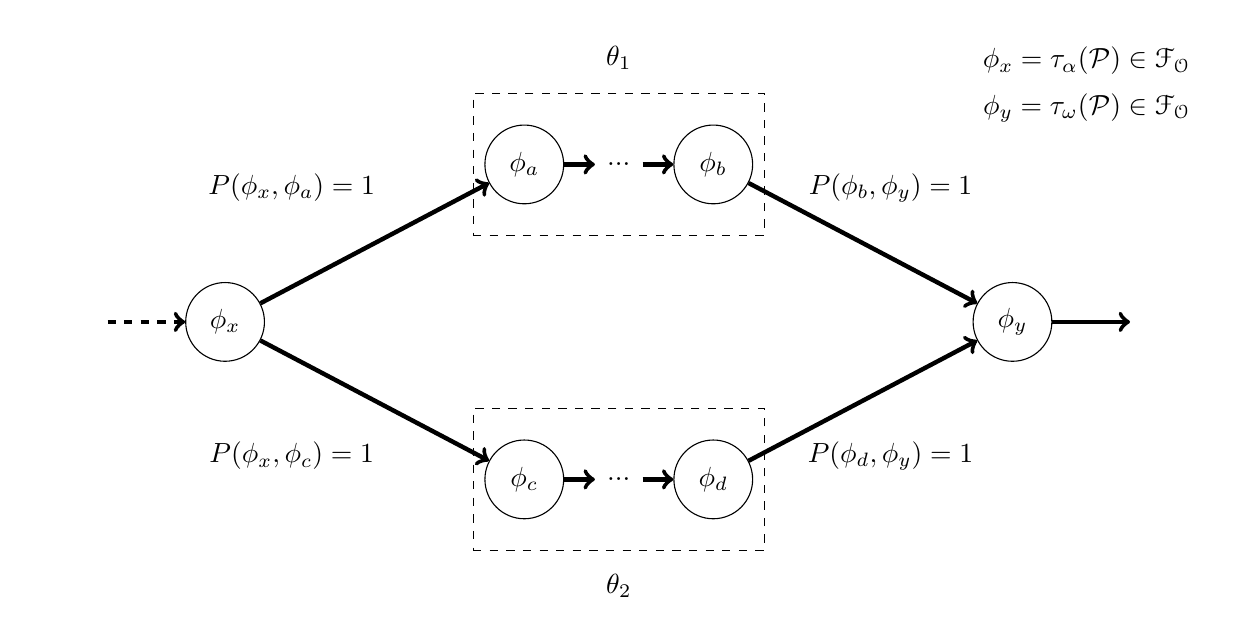
\begin{tikzpicture}
		
		
		\node[circle,draw=white,minimum width = 1cm] 
		(start) at (-2,0) {};
		
		\node[circle,draw=white,minimum width = 1cm] 
		(end) at (12,0) {};
		
		\node[circle, draw, minimum width = 1cm]        					   
		(branchStartNode) at (0,0) {$\phi_x$};
		
		\node[circle, draw, minimum width = 1cm]        					   
		(branchEndNode) at (10,0) {$\phi_y$};
		
		
		\node[circle, draw, minimum width = 1cm]        					   
		(Node1) at (3.8,2) {$\phi_a$};
		
		\node[circle, minimum width = 0.3cm]       					   
		(Node2) at (5,2) {...};
		
		\node[circle, draw, minimum width = 1cm]       					   
		(Node3) at (6.2,2) {$\phi_b$};
		
		\node[circle, draw, minimum width = 1cm]       					   
		(Node4) at (3.8,-2) {$\phi_c$};
		
		\node[circle, minimum width = 0.3cm]       					   
		(Node5) at (5,-2) {...};
		
		\node[circle, draw, minimum width = 1cm]       					   
		(Node6) at (6.2,-2) {$\phi_d$};
		
		\draw[ultra thick,->] (branchStartNode) edge node[xshift=-30 ,yshift=20]{$P(\phi_x,\phi_a) = 1$} (Node1);
		
		\draw[ultra thick,->] (branchStartNode) edge node[xshift=-30 ,yshift=-20]{$P(\phi_x,\phi_c) = 1$} (Node4);
		
		\draw[ultra thick,->] (Node3) edge node[xshift=10 ,yshift=20]{$P(\phi_b,\phi_y) = 1$} (branchEndNode);
		
		\draw[ultra thick,->] (Node6) edge node[xshift=10 ,yshift=-20]{$P(\phi_d,\phi_y) = 1$} (branchEndNode);
		
		% Dashed lines
		
		\draw[dashed,ultra thick, ->] (start) -- (branchStartNode);
		
		\draw[ultra thick, ->] (branchEndNode) -- (end);
		
		\draw[ultra thick, ->] (Node1) -- (Node2);
		
		\draw[ultra thick, ->] (Node2) -- (Node3);
		
		\draw[ultra thick, ->] (Node4) -- (Node5);
		
		\draw[ultra thick, ->] (Node5) -- (Node6);
		
		% Frames
		
		\node[rectangle, draw, dashed, minimum width =3.7cm, minimum height=1.8cm] (sub1) at (5,2) {};
		\node[circle,above of=sub1, yshift=10] (label1) {$\theta_1$};
		
		\node[rectangle, draw, dashed, minimum width =3.7cm, minimum height=1.8cm] (sub2) at (5,-2) {};
		\node[circle,below of=sub2, yshift=-10] (label2) {$\theta_2$};
		
		legend
		
		\matrix [below left] at (current bounding box.north east) {
			\node [] {$\phi_x = \tau_{\alpha}(\mathcal{P}) \in \mathscr{F_O}$}; \\
			\node [] {$\phi_y = \tau_{\omega}(\mathcal{P}) \in \mathscr{F_O}$}; \\
		};
		
		
	\end{tikzpicture}
	\caption{Parallel structure in the serverless workflow.}
\end{figure}

Clearly, the response time of a parallel structure is equal to the longest response time of all its sub-choreographies.

Formally, let $\theta_i \in \Theta$ the $i$-th sub-choreography of $\mathcal{P}$, where $i \in \N \cap \left[1,n\right]$, and $\textbf{X} \in \Omega$ a choreography configuration.

At any time $t$, the response time and the cost of $\mathcal{P}$ can be computed as follows:

\begin{equation}
	RT_{parallel}(\textbf{X}, t) \mathDef max \left\lbrace RT_C(\textbf{X}, \theta_i, t) \mid \theta \in \Theta \right\rbrace 
\end{equation}

\begin{equation}
	C_{parallel}(\textbf{X}, t) \mathDef \sum_{i = 1}^n P(\phi_{x}, \alpha(\theta_i)) \cdot C_C(\textbf{X}, \theta_i, t)
\end{equation}

We always assume that the exit probability of the a parallel structure is zero. Formally

\begin{equation}
	P_{exit}^{(parallel)}(t) \mathDef 0
\end{equation}


During choreography simplification process, a parallel structure can be replaced by a fake executable function $\phi \in \mathscr{F_E}$ whose response time and cost are equal to $RT_{parallel}(\textbf{X}, t)$ and $RT_{parallel}(\textbf{X}, t)$ respectively.

\subsubsection{Branch}

Let $\mathcal{B} = (\Phi,E,\Theta)$ a structure and suppose that $\tau_{\alpha}(\mathcal{B}) = \phi_{x}$ and $\tau_{\omega} (\mathcal{B}) = \phi_{y}$. 

$\mathcal{B}$ is called ``\textit{branch structure}'' when following conditions are hold:

\begin{eqnarray}
	TPP(\pi) \neq 1  & \qquad \forall \pi \in \Pi(\phi_{x}, \phi_{y}) \\
	|\Theta| = n  & \qquad n \in \N \setminus \left\{0\right\} \\
	E[I_{\theta}] = 1 & \qquad \forall \theta \in \Theta \\
	P_{exit}^{(C)}(t) \neq 0 & \qquad \forall \theta \in \Theta
\end{eqnarray}

\begin{figure}[h!]
	\centering
	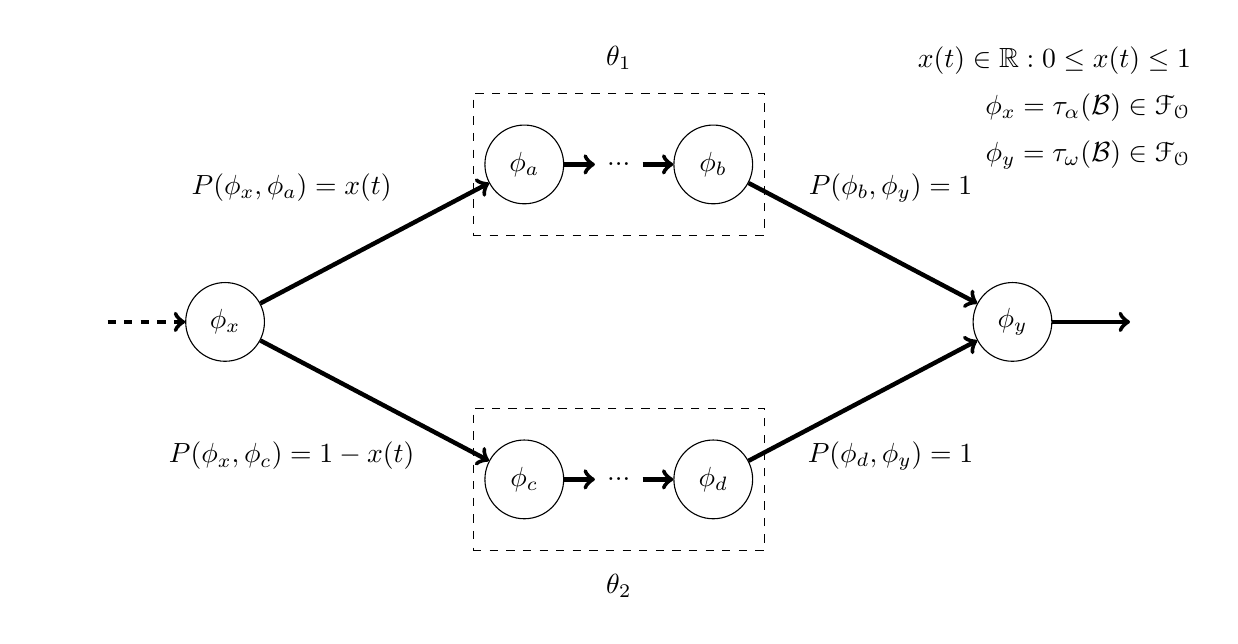
\begin{tikzpicture}
		
		
		\node[circle,draw=white,minimum width = 1cm] 
		(start) at (-2,0) {};
		
		\node[circle,draw=white,minimum width = 1cm] 
		(end) at (12,0) {};
		
		\node[circle, draw, minimum width = 1cm]        					   
		(branchStartNode) at (0,0) {$\phi_x$};
		
		\node[circle, draw, minimum width = 1cm]        					   
		(branchEndNode) at (10,0) {$\phi_y$};
		
		
		\node[circle, draw, minimum width = 1cm]        					   
		(Node1) at (3.8,2) {$\phi_a$};
		
		\node[circle, minimum width = 0.3cm]       					   
		(Node2) at (5,2) {...};
		
		\node[circle, draw, minimum width = 1cm]       					   
		(Node3) at (6.2,2) {$\phi_b$};
	
		\node[circle, draw, minimum width = 1cm]       					   
		(Node4) at (3.8,-2) {$\phi_c$};
		
		\node[circle, minimum width = 0.3cm]       					   
		(Node5) at (5,-2) {...};
		
		\node[circle, draw, minimum width = 1cm]       					   
		(Node6) at (6.2,-2) {$\phi_d$};
		
		\draw[ultra thick,->] (branchStartNode) edge node[xshift=-30 ,yshift=20]{$P(\phi_x,\phi_a) = x(t)$} (Node1);
		
		\draw[ultra thick,->] (branchStartNode) edge node[xshift=-30 ,yshift=-20]{$P(\phi_x,\phi_c) = 1-x(t)$} (Node4);
		
		\draw[ultra thick,->] (Node3) edge node[xshift=10 ,yshift=20]{$P(\phi_b,\phi_y) = 1$} (branchEndNode);
		
		\draw[ultra thick,->] (Node6) edge node[xshift=10 ,yshift=-20]{$P(\phi_d,\phi_y) = 1$} (branchEndNode);
		
		% Dashed lines
		
		\draw[dashed,ultra thick, ->] (start) -- (branchStartNode);
		
		\draw[ultra thick, ->] (branchEndNode) -- (end);
		
		\draw[ultra thick, ->] (Node1) -- (Node2);
		
		\draw[ultra thick, ->] (Node2) -- (Node3);
		
		\draw[ultra thick, ->] (Node4) -- (Node5);
		
		\draw[ultra thick, ->] (Node5) -- (Node6);
		
		% Frames
		
		\node[rectangle, draw, dashed, minimum width =3.7cm, minimum height=1.8cm] (sub1) at (5,2) {};
		\node[circle,above of=sub1, yshift=10] (label1) {$\theta_1$};
		
		\node[rectangle, draw, dashed, minimum width =3.7cm, minimum height=1.8cm] (sub2) at (5,-2) {};
		\node[circle,below of=sub2, yshift=-10] (label2) {$\theta_2$};
		
		legend
		
		\matrix [below left] at (current bounding box.north east) {
			\node [] {$x(t) \in \mathbb{R} : 0 \leq x(t) \leq 1$}; \\
			\node [] {$\phi_x = \tau_{\alpha}(\mathcal{B}) \in \mathscr{F_O}$}; \\
			\node [] {$\phi_y = \tau_{\omega}(\mathcal{B}) \in \mathscr{F_O}$}; \\
		};
		
		
	\end{tikzpicture}
	\caption{Branch/Switch structure in the serverless workflow.}
\end{figure}

Let $\theta_i \in \Theta$ the $i$-th sub-choreography of $\mathcal{B}$, where $i \in \N \cap \left[1,n\right]$. At any time $t$, the response time and the cost of the branch structure $\mathcal{B}$ can be computed as follows:

\begin{equation}
	RT_{branch}(\textbf{X}, t) \mathDef \sum_{i = 1}^n P(\phi_{x}, \alpha(\theta_i)) \cdot  RT_C(\textbf{X}, \theta_i, t)
\end{equation}

\begin{equation}
	C_{branch}(\textbf{X}, t) \mathDef \sum_{i = 1}^n P(\phi_{x}, \alpha(\theta_i)) \cdot C_C(\textbf{X}, \theta_i, t)
\end{equation}

The exit probability of the a branch/switch structure can be computed as follows:

\begin{equation}
	P_{exit}^{(branch)} \mathDef \sum_{i = 1}^n P(\phi_{x}, \alpha(\theta_i)) \cdot P_{exit}(\theta_i, t)
\end{equation}

\subsubsection{Loop}

Let $\mathcal{L} = (\Phi,E,\Theta)$ a structure and suppose that $\tau_{\alpha}(\mathcal{L}) = \phi_{x}$ and $\tau_{\omega} (\mathcal{L}) = \phi_{y}$. 

Being $\theta \in \Theta$ the unique sub-choreography of $\mathcal{L}$, the structure $\mathcal{L}$ is called ``\textit{loop structure}" when following conditions are hold:

\begin{eqnarray}
	TPP(\pi) = 1 & \qquad \forall \pi \in \Pi(\phi_{x}, \phi_{y}) \\
	|\Theta| = 1  &  \\
	P(\phi_{x}, \alpha(\theta)) = x(t) & \\
	P(\phi_{x}, \phi_{y}) = 1 - x(t) & \\
	P(\phi_{c}, \phi_{z}) = 1 & \phi_{c} \in \omega(\theta)\\
\end{eqnarray}

\begin{figure}[h!]
	\centering
	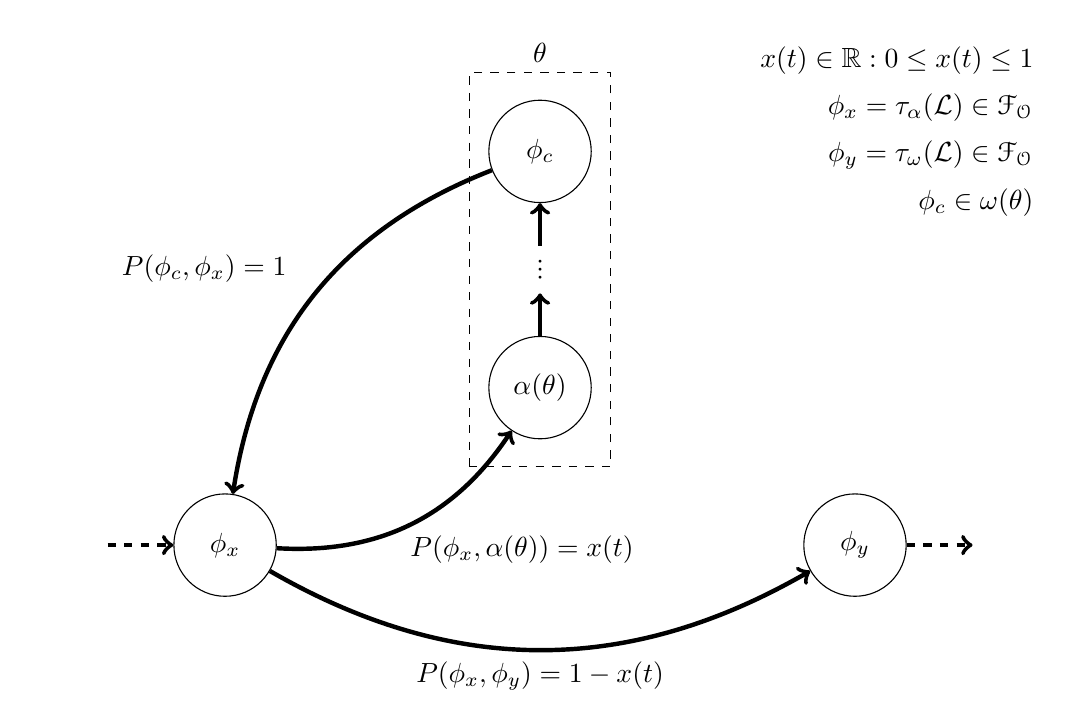
\begin{tikzpicture}
		
		
		\node[circle,draw=white,minimum width = 1cm] 
		(start) at (-2,0) {};
		
		\node[circle,draw=white,minimum width = 1cm] 
		(end) at (10,0) {};
		
		\node[circle, draw, minimum width = 1.3cm]        					   
		(startLoopNode) at (0,0) {$\phi_x$};
		
		\node[circle, draw, minimum width = 1.3cm]        					   
		(endLoopNode) at (8,0) {$\phi_y$};
	
		\node[circle, draw, minimum width = 1.3cm]        					   
		(node1) at (4,2) {$\alpha(\theta)$};
		
		\node[circle, minimum width = 0.5cm, rotate=90]        					   
		(node2) at (4,3.5) {...};
		
		\node[circle, draw, minimum width = 1.3cm]        					   
		(node3) at (4,5) {$\phi_c$};
	
		% Edges...
	
		\draw[bend right,below, ultra thick,->] (startLoopNode) edge node[xshift=40]{$P(\phi_x,\alpha(\theta)) = x(t)$} (node1);
		
		\draw[bend right,above, ultra thick,->] (node3) edge node[xshift=-40]{$P(\phi_c,\phi_x) = 1$} (startLoopNode);
		
		\draw[bend right,below, ultra thick,->] (startLoopNode) edge node[]{$P(\phi_x,\phi_y) = 1 - x(t)$} (endLoopNode);
		
		
		
		\draw[dashed,ultra thick, ->] (start) -- (startLoopNode);
		\draw[dashed,ultra thick, ->] (endLoopNode) -- (end);
		
		
		\draw[ultra thick, ->] (node1) -- (node2);
		\draw[ultra thick, ->] (node2) -- (node3);
		
		% Frames
		
		\node[rectangle, draw, dashed, minimum width =1.8cm, minimum height=5cm] (sub1) at (4,3.5) {};
		\node[circle,above of=sub1, yshift=50] (label1) {$\theta$};
	
		%legend
	
			\matrix [below left] at (current bounding box.north east) {
			\node [] {$x(t) \in \mathbb{R} : 0 \leq x(t) \leq 1$}; \\
			\node [] {$\phi_x = \tau_{\alpha}(\mathcal{L}) \in \mathscr{F_O}$}; \\
			\node [] {$\phi_y = \tau_{\omega}(\mathcal{L}) \in \mathscr{F_O}$}; \\
			\node [] {$\phi_c \in \omega(\theta)$}; \\
		};
		
	\end{tikzpicture}
	\caption{Parallel structure in the serverless workflow.}
\end{figure}

In order to compute performance data of a loop structure, $E[I_{\theta}]$, that is the expected value of the number of iterations of $\mathcal{L}$, is required.

To compute aforementioned information, we can model our problem using geometric distribution, which gives the probability according to which the first occurrence of success requires $k \in \N$ independent trials, each with success probability $p$ and failure probability $q = 1 - p$. In our case, if the our success corresponds to event ``\textit{we will not execute the loop body}", we know that success probability $p$ is given by:

\begin{eqnarray}
	p = P(\phi_x,\phi_y) = 1 - P\Big(\phi_{x}, \alpha(\theta)\Big) \\
\end{eqnarray}

Then:

\begin{eqnarray}
	P(I_{\theta} = k) & = & p \cdot (1-p)^{k-1} \\
	& = & pq^{k-1} \\
	& = & \Big[  1 - P\Big(\phi_{x}, \alpha(\theta)\Big) \Big] \cdot \bigg[  P\Big(\phi_{x}, \alpha(\theta)\Big) \bigg] ^{k-1} \\
\end{eqnarray}

\begin{eqnarray}
	E[I_{\theta}] & = & \sum_{k = 1}^\infty (k-1) pq^{k-1} \nonumber \\
	& = & p \sum_{k = 0}^\infty kq^{k} \nonumber \\
	& = & p \cdot \frac{q}{(1-q)^2} \nonumber \\
	& = & \dfrac{q}{p} \nonumber \\
	& = & \dfrac{P\Big(\phi_{x}, \alpha(\theta)\Big)}{1 - P\Big(\phi_{x}, \alpha(\theta)\Big)} 
\end{eqnarray}

More precisely, at any time $t$, the expected value regarding the number of iterations of $\mathcal{L}$, involving the execution of the sub-choreography $\theta$, can be computed as follows:

\begin{equation}
	E[I_{\theta}](t) = \dfrac{x(t)}{1 - x(t)}
\end{equation}


At any time $t$, the response time and the cost of the loop structure $\mathcal{L}$ can be computed as follows:

\begin{equation}
	RT_{loop}(\textbf{X}, t) \mathDef E[I_{\theta}](t) \cdot  RT_C(\textbf{X}, \theta, t)
\end{equation}

\begin{equation}
	C_{loop}(\textbf{X}, t) \mathDef E[I_{\theta}](t) \cdot C_C(\textbf{X}, \theta, t)
\end{equation}

The exit probability of the a loop structure can be computed as follows:

\begin{equation}
	P_{exit}^{(loop)} \mathDef E[I_{\theta}](t) \cdot P_{exit}(\theta, t)
\end{equation}

\section{Optimization Problem Formulations}

To achieve our goal consisting in to find the best choreography configuration capable to guarantee QoS constraints imposed by an user, we have to solve an optimization problem, which we have formulated in two very different manners, where:

\begin{itemize}
	\item the first one is based on the Multidimensional Knapsack Problem formulation.
	\item the second one is based on the multi-dimensional multi-choice knapsack problem formulation. 
\end{itemize}

In this section, we will describe and analyze both approach, despite only for the second one we have developed and implemented an heuristic approach capable to solve it in a faster way respect to exact algorithms. 

\subsection{Multidimensional Knapsack Problem Formulation}

Let $\mathcal{C} = (\Phi,E)$ a serverless choreography, $\textbf{X} \in \Omega$ a choreography configuration and $\left\langle (RT,w_{RT}),(C,w_{C}) \right\rangle$ the SLA imposed by an user regarding the execution of $\mathcal{C}$

At any time $t$, the \textit{score} $S(\textbf{X},t)$, or \textit{profit}, of the choreography configuration $\textbf{X}$ can be computed as follows:

\begin{equation}
	S(\textbf{X},t) \mathDef w_{RT} \cdot \dfrac{RT_{C_{\textbf{max}}}(t) - RT_C(\textbf{X},t)}{RT_{C_{\textbf{max}}}(t) - RT_{C_{\textbf{min}}}(t)} + w_{C} \cdot \dfrac{C_{C_{\textbf{max}}}(t) - C_C(\textbf{X},t)}{C_{C_{\textbf{max}}}(t) - C_{C_{\textbf{min}}}(t)}
\end{equation}

where:

\begin{itemize}
	\item $RT_{C_{\textbf{max}}}(t)$ ($RT_{C_{\textbf{min}}}(t)$) and $C_{C_{\textbf{max}}}(t)$ ($C_{C_{\textbf{min}}}(t)$) denote, respectively, the maximum (minimum) value for the overall expected response time and cost observed at time $t$.
\end{itemize}

A very naive formulation to our problem can be expressed in term of the the Multidimensional Knapsack Problem (MKP), a well-studied, strongly NP-hard combinatorial optimization problem occurring in many different applications, whose goal is to choose a subset of items with maximum total profit. Selected items must, however, not exceed resource capacities, which are called as knapsack constraints.

The MKP formulation for our problem can be defined by the following ILP:

\begin{align}
\displaystyle max \qquad & \displaystyle \sum_{\omega = 1}^{|\Omega|} x_{\omega} F(\textbf{X}_{\omega}) \\
\text{subject to} \qquad & \displaystyle \sum_{\omega = 1}^{|\Omega|} x_{\omega} C(\textbf{X}_{\omega}) \leq C_{user} \\
& \displaystyle \sum_{\omega = 1}^{|\Omega|} x_{\omega} RT(\textbf{X}_{\omega}) \leq RT_{user} \\ 
& \displaystyle \sum_{\omega = 1}^{|\Omega|} x_{\omega} = 1 & \\
& x_{\omega} \in \lbrace 0, 1 \rbrace & \qquad \forall \omega \in \N \cap [1,|\Omega|]
\end{align}

where:

Is very important to observe, that each column of above formulation represents the profit and resource requirements referring to a choreography configuration.

The number of existing choreography configuration (or columns above LP) is very large because it grows exponentially. Therefore, become impractical to generate and enumerate all possible choreography configuration.

For example, suppose to have a serverless choreography $\mathcal{C}$ made up of $6$ executable functions. Supposing to have $46$ possible memory choices, even if only one concrete function exist for each executable function, the solution space $\Omega$ will contain $9.47$ billion different configurations, making any exhaustive enumeration and search computationally unfeasible. 

Even if we had a way of generating all configurations, that is all columns of our problem, due to its complexity, any attempt to find the optimal solution rapidly will be an illusion. Moreover, it will be very likely that any computer runs out his memory.

\subsection{Multi-dimensional Multi-choice Knapsack Problem Formulation}

To avoid the enumeration of all possible choreography configuration, we have decided to use another kind of formulation, which is base on the Multidimensional Multiple-choice Knapsack Problem (MMKP), a variant of the previous one. 

Let $\mathcal{C} = (\Phi,E)$ a choreography and $\mathscr{F_E}(\mathcal{C})$ the set containing all executable functions of $\mathcal{C}$. Moreover, suppose that $|\mathscr{F_E}(\mathcal{C})| = n \in \N \setminus \left\{0\right\}$.

In this context, we have $n$ \textit{groups} of \textit{items} where, for $i \in \N \cap \left[1,n\right]$, the $i$-th group represents the set of all possible executable configurations for the executable function $\phi_i \in \mathscr{F_E}(\mathcal{C})$, which belong to the set $\left\{ \textbf{F}_{\phi_{i}} \times \N \right\}$, where $\textbf{F}_{\phi_{i}}$, we recall, is the implementation-set for $\phi_i$. Therefore, each $i$-th group contains $|\left\{ \textbf{F}_{\phi_{i}} \times \N \right\}|$ items, that is executable function configurations.

According to MMKP, our objective is to pick exactly one item from each group, that is exactly one configuration for each executable function $\phi \in \mathscr{F_E}(\mathcal{C})$, in such a way to maximize the profit value of the selected items, respecting several resource constraints of the knapsack, which, in our case, are represented by SLAs attributes values imposed by users. 

\subsubsection{Profit and resource requirement computation}

Before to formulate our MMKP instance, we have to explain how we can compute profit and resource requirements, expressed in term of response time and cost, for each executable function configuration belonging to each group, which is somewhat complicated.

Firstly, we recall that the notation $x_{\phi_{i_{j}}} = (f_j, m_j) $ represents an executable function configuration for the executable function $\phi_i \in \mathscr{F_E}(\mathcal{C})$, for some $i \in \N \cap [1,|\mathscr{F_E}(\mathcal{C})|]$ and $j \in \N \cap [1,|\textbf{F}_{\phi_{i}} \times \N|]$. 

Let's now define some notations:

\begin{itemize}
	\item For some $m \in \N$, $\widehat{\theta_k}^{(\phi_i)} \mathDef {\theta^{(\phi_i)}_1, \ldots, \theta^{(\phi_i)}_m}$ represents the sequence of all sub-choreographies of $\mathcal{C}$ such that:
	
	\begin{equation}
		\phi_i \in \mathscr{F_E}(\theta^{(\phi_i)}_1)
	\end{equation}
	
	\begin{equation}
		\theta^{(\phi_i)}_n = \mathcal{C}
	\end{equation}
	
	\begin{equation}
		\theta^{(\phi_i)}_k \text{ is a sub-choreography of } \theta^{(\phi_i)}_{k+1} \qquad \forall k \in \left[1;m-1\right]
	\end{equation}

\item $E[I_{\phi_i}]$ represents the expected value of the number of invocations of the executable function $\phi_i$, which can be defined as follows.

\begin{equation}	
	E[I_{\phi_i}] \mathDef \left\{
	\begin{array}{lcr}
		1 & \text{\textit{if}} & m = 1 \\ 
		\displaystyle \prod_{k = 2}^m E[I_{\theta_{k-1}^{(\phi_i)}}] & \text{\textit{if}} & m \geq 2 \\
	\end{array} \right.
\end{equation}



\item For some $k \in \N \cap \left[1;m-1\right]$, $P_{exe}^C(\theta^{(\phi_i)}_k)$ is the probability to execute the entry point $\alpha(\theta^{(\phi_i)}_k)$ of the choreography $\theta^{(\phi_i)}_k$, when the function $pred(\alpha(\theta^{(\phi_i)}_k))$ is executed. 

That probability can be computed as follows:

\begin{equation}	
	P_{exe}^C(\theta^{(\phi_i)}_k) \mathDef \left\{
	\begin{array}{lcr}
		1 & \text{\textit{if}} & m = 1 \\ 
		P \bigg(  pred\Big( \alpha(\theta^{(\phi_i)}_{k}) \Big), \alpha(\theta^{(\phi_i)}_{k}) \bigg) & \text{\textit{if}} & m \geq 2 \\
	\end{array} \right.
\end{equation}


\item For some $k \in \N \cap \left[1;m-1\right]$, $P_{exe}^{F}(\theta_k, \phi)$ is the probability to execute the function $\phi \in \mathscr{F_E}(\theta_k)$ when the abstract function $\alpha(\theta_k)$ is executed. 

Let $\Pi(\alpha(\theta_k),\phi)$ the set containing all possible paths starting from the entry point of $\theta_k$ to $\phi$. Aforementioned probability can be computed using following formula:

\begin{equation}
	P_{exe}^{F}(\theta_k, \phi) \mathDef \prod_{ \phi_k \in \Pi(\alpha(\theta_k),\phi) \cap \mathscr{F_O}(\theta_k)} (1 - P_{exit}(\phi_k))
\end{equation}

\end{itemize}

Defining the quantity $\Gamma_{\theta_y^{(\phi_{i})}}$, as the probability to execute the entry point of the sub-choreography $\theta_y^{(\phi_{i})}$ as follows:

\begin{equation}
	\Gamma_{\theta_y^{(\phi_{i})}} \mathDef \prod_{k = y + 1}^{m}  P_{exe}^C(\theta^{(\phi_i)}_{k-1}) \cdot P_{exe}^{F}(\theta^{(\phi_i)}_{k}, pred(\alpha(\theta^{(\phi_i)}_{k-1})))
\end{equation}

we can compute resource requirements $c_{\phi_{i_{j}}}$ and $t_{\phi_{i_{j}}}$ in the following ways:


\begin{eqnarray}
	c_{\phi_{i_{j}}} & \mathDef & \left\{ 
	\begin{array}{lcl}
		C_{avg}(x_{\phi_{i_{j}}}) \cdot P_{exe}^{F}(\theta^{(\phi_i)}_1, \phi_i) & \text{\textbf{if}} & m = 1 \\ 
		\displaystyle C_{avg}(x_{\phi_{i_{j}}}) \cdot P_{exe}^{F}(\theta^{(\phi_i)}_1, \phi_i) \cdot E[I_{\phi_i}] \cdot \Gamma_{\theta_1^{(\phi_{i})}} & \text{\textbf{if}} & m \geq 2 \\ 
	\end{array} \right.
\end{eqnarray}

\begin{eqnarray}
	t_{\phi_{i_{j}}} & \mathDef & \left\{ 
	\begin{array}{lcl}
		T_{avg}(x_{\phi_{i_{j}}}) \cdot P_{exe}^{F}(\theta^{(\phi_i)}_1, \phi_i) & \text{\textbf{if}}  & m = 1 \\ 
		\displaystyle T_{avg}(x_{\phi_{i_{j}}}) \cdot P_{exe}^{F}(\theta^{(\phi_i)}_1, \phi_i) \cdot E[I_{\phi_i}] \cdot \Gamma_{\theta_1^{(\phi_{i})}} & \text{\textbf{if}} & m \geq 2 \\ 
	\end{array} \right.
\end{eqnarray}





Finally, for any executable function configuration $x_{\phi_{i_j}}$, its profit $p_{\phi_{i_{j}}}$ is determined as follows;

\begin{equation}
	p_{\phi_{i_{j}}} \mathDef w_{RT} \cdot \dfrac{t_{\phi_{i_{\textbf{MAX}}}} - t_{\phi_{i_{j}}}}{t_{\phi_{i_{\textbf{MAX}}}} - t_{\phi_{i_{\textbf{MIN}}}}} + w_{C} \cdot \dfrac{c_{\phi_{i_{\textbf{MAX}}}} - c_{\phi_{i_{j}}}}{c_{\phi_{i_{\textbf{MAX}}}} - c_{\phi_{i_{\textbf{MIN}}}}}
\end{equation}

where:

\begin{itemize}
	\item $t_{\phi_{i_{\textbf{MIN}}}}$ and $t_{\phi_{i_{\textbf{MAX}}}}$ represent, respectively, the minimum and maximum response time values regarding the execution of all concrete function implementing $\phi_i$. 
	
	In other words, they represent the minimum and maximum resource requirement, referring to the response time, of all items belonging to the $i$-th group of our problem.
	
	\item $c_{\phi_{i_{\textbf{MIN}}}}$ and $c_{\phi_{i_{\textbf{MAX}}}}$ represent, respectively, the minimum and maximum cost values spent by all concrete function implementing $\phi_i$.
\end{itemize}

From now, we will use $\mathcal{\widetilde{P}}$ to denote the set containing all parallel structures of $\mathcal{C}$, while $\mathcal{\widetilde{P}}_i$ represents the $i$-th parallel structure belonging to $\mathcal{\widetilde{P}}$ for $i \in \N \cap \left[1;p \right]$, where $p = |\mathcal{\widetilde{P}}|$. Clearly, the notation $\mathscr{F_E}(\mathcal{\widetilde{P}})$ represents the set of all executable functions contained inside any parallel structure of a given choreography.

We will use $\Delta_{\mathcal{\widetilde{P}}_{i_j}}$ notation to represent the set containing all executable functions $\phi \in \mathscr{F_E}(\theta_{i_j})$, where $\theta_{i_j}$ is the $j$-th sub-choreography of the parallel structure $\mathcal{\widetilde{P}}_i$, which can be formally defined as follows:

\begin{equation}
	\Delta_{\mathcal{\widetilde{P}}_{i_j}} \mathDef \left\{ \phi \in \mathscr{F_E}(\mathcal{C}) \cap \mathscr{F_E}(\theta_{i_j}) : \text{  $\theta_{i_j}$ is the $j$-th sub-choreography of } \mathcal{\widetilde{P}}_i \right\} 
\end{equation}

In this context, $\Delta_{\mathcal{\widetilde{P}}_{i_j}}$ can be viewed as one of the parallel paths of $\mathcal{\widetilde{P}}_i$. Since the actual response time of any sub-choreography of $\mathcal{\widetilde{P}}_i$ depend on to the slower sub-choreography of $\mathcal{\widetilde{P}}_i$, can be not trivial to compute the profit and resource requirements for every function inside a parallel structure.  

Therefore, the main idea, regarding profit and resource requirements computation, is to verify if, for every parallel path for every parallel structure of the choreography, resource requirements are respected. 

We will use $\Xi$ to denote the set of all possible parallel paths combination inside a choreography. Formally it can be defined as follows: 

\begin{eqnarray}
	\Xi & \mathDef & \left\lbrace \Delta_{\mathcal{\widetilde{P}}_{1}}, \ldots, \Delta_{\mathcal{\widetilde{P}}_{p}} \right\rbrace \nonumber \\ 
	& \in & \left\{  \left\{ \bigcup_{j=1}^{|\mathcal{\widetilde{P}}_i|} \Delta_{\mathcal{\widetilde{P}}_{1_j}} \right\} \times \ldots \times \left\{ \bigcup_{j=1}^{|\mathcal{\widetilde{P}}_p|} \Delta_{\mathcal{\widetilde{P}}_{p_j}} \right\} \right\}  \nonumber \\
	& = & \Cross_{i = 1}^p  \left\{ \bigcup_{j=1}^{|\mathcal{\widetilde{P}}_i|} \Delta_{\mathcal{\widetilde{P}}_{i_j}} \right\}  \nonumber \\
\end{eqnarray}

In this context, any $\xi \in \Xi$ represents a set of executable functions belonging to an unique combinations of parallel paths.

\subsubsection{Formulation}

Finally, wa are able to formulate our MMKP instance problem, which can be expressed as follows:

\begin{align}
	\label{MMKP}
	\displaystyle max \quad & \displaystyle \sum_{i = 1}^{|\mathscr{F_E}|}  \sum_{j = 1}^{|\textbf{F}_{\phi_{i}} \times \N|} y_{\phi_{i_{j}}} p_{\phi_{i_{j}}} & \\	
	\text{subject to} \quad  & \displaystyle \sum_{i = 1}^{|\mathscr{F_E}|}  \sum_{j = 1}^{|\textbf{F}_{\phi_{i}} \times \N|} y_{\phi_{i_{j}}} c_{\phi_{i_{j}}} \leq C_{user} & \\
	& \displaystyle \sum_{\phi_i \in \mathscr{F_E} \cap \mathscr{F_E}(\mathcal{\widetilde{P}})}  \sum_{j = 1}^{|\textbf{F}_{\phi_{i}} \times \N|} y_{\phi_{i_{j}}} t_{\phi_{i_{j}}} + \nonumber \\
	& \qquad + \sum_{\phi_h \in \xi}  \sum_{j = 1}^{|\textbf{F}_{\phi_{h}} \times \N|} y_{\phi_{h_{j}}} t_{\phi_{h_{j}}} \leq RT_{user} & 
	\forall \xi \in \Xi \\	
	& \displaystyle \sum_{j = 1}^{|\textbf{F}_{\phi_{i}} \times \N|} y_{\phi_{i_{j}}} = 1 & \forall i \in \N \cap \left[ 1, |\mathscr{F_E}| \right] \\
	& y_{\phi_{i_{j}}} \in \lbrace 0, 1 \rbrace &
	\begin{array}{r}
		\forall i \in \N \cap \left[ 1, |\mathscr{F_E}| \right] \\ \forall j \in \N \cap [1,|\textbf{F}_{\phi_{i}} \times \N|]
	\end{array}
\end{align}


To simplify our notations, from now, we will use $o_{i_j}$ notation to denote the $i$-th item belonging to the $j$-th group, the latter denoted with $g_i$; clearly, in our context, the item $o_{i_j}$ coincides with the $j$-th executable function configuration $x_{\phi_{i_j}}$ for the executable function $\phi_i \in \mathscr{F_E}(\mathcal{C})$, for some $i \in \N \cap [1,|\mathscr{F_E}(\mathcal{C})|]$ and $j \in \N \cap [1,|\textbf{F}_{\phi_{i}} \times \N|]$. 

A solution of a MMKP is a set of selected objects $S \mathDef \left\{o_{1}, \ldots o_{n} \right\}$ where, clearly, an object $o_{i_j}$ is selected if the corresponding decision variable $y_{\phi_{i_j}}$ has been set to 1.


\subsubsection{The heuristic approach based on ACO}

Being MMKP an NP-hard problem, it is not always possible to find a feasible solution in a reasonable computing time especially for big instances, therefore an heuristic approach is needed for solving it. 

We have decided to built an algorithm based on \textit{Ant Colony Optimization} (ACO), a class of stochastic meta-heuristics that have been applied to solve many combinatorial optimization problems such as traveling salesman problems, quadratic assignment problems, or vehicle routing problems. 

Aforementioned class of meta-heuristics imitate the behavior shown by real ants when searching for food, where many simple interactions between single ants result in a very complex behavior of the whole ant colony.

Any ACO algorithm is based on a set of computational agent, called \textit{artificial ants}, which iteratively constructs a so-called  \textit{partial solution} for the instance to solve. At each iteration, each artificial ant moves from a partial solution to another, applying a series of stochastic local decisions whose policy is based on following parameters:

\begin{description}
	\item[Attractiveness] which is a value computed using an heuristic approach indicating the a \textit{priori} desirability of a given partial solution.
	
	\item[Pheromone Trail] which represents a value indicating how proficient it has been in the past to select a particular partial solution, representing, therefore, an a \textit{posteriori} indication of its desirability.
\end{description} 

In very simple terms, each ant incrementally constructs the partial solution to the problem and, after evaluating the find solution, it modifies the pheromone trail on the components used in its solution; that pheromone information will be use by future ants to find a better solutions to the problem instance. In fact, by increasing or decreasing the level of pheromone trails, ants distinguish "\textit{good}" from "\textit{bad}" solutions. In other words, pheromone trails represent the way according to which each ants communicate in order to find the best solution.
 
\subsubsection{Definition}

To solve MMKPs with ACO, we have to define how pheromone trails are laid by artificial ants, explaining how they follow them when constructing new partial solutions. In other words we need to decide which components of the constructed solutions should be rewarded, and how to exploit these rewards when constructing new solutions.

We define the \textit{solution's components graph} $\mathcal{G}=(\textbf{O},\textbf{E})$, on which ants lay pheromone trails, as a directed weighted graph such that:

\begin{equation}
	\textbf{O} \mathDef \bigcup_{j=1}^n \bigcup_{j=1}^{|g_i|} \left\{ o_{i_j} \right\}
\end{equation}

\begin{equation}
	(o_{i_j}, o_{k_m}) \in E \Leftrightarrow i \neq k \qquad \forall i,k \in \N \cap \left\{1,n\right\}, \forall m,j \in \N
\end{equation}

where: 

\begin{itemize}
	
	\item The set of vertices $\textbf{O}$ is made up all items belonging to each group. 
	
	Moreover, any object $o_{i_j}$ is adjacent to all other objects belonging to any group except those which belong to its same group.
	
	\item The weight $w \in \Rplus$ associated to each edge $(o_{i_j}, o_{k_m}) \in \textbf{E}$ is the value of the \textit{pheromone trail} laid by our artificial ants and it can change during algorithm execution. 
	
	The value of pheromone trail associated to each edge $(o_{i_j}, o_{k_m})$ during the $k$-th iteration of the algorithm is denoted as follows:
	
	\begin{equation}
		\tau_k(o_{i_j}, o_{k_m}) = w_k
	\end{equation}
	
	Intuitively, the pheromone value associated to the edge $(o_{i_j}, o_{k_m}) \in E$ represents the desirability to select the object $o_{k_m}$ when $o_{i_j}$ was been previously selected as part of the solution.
	
	We have adopted the so-called $\mathcal{MAX} - \mathcal{MIN}$ Ant System, according to which following constrain must be hold:
	
	\begin{equation}
		w_{\textbf{min}} \leq w_k \leq w_{\textbf{max}} 
	\end{equation}

	\begin{equation}
		\tau_0(o_{i_j}, o_{k_m}) = w_{\textbf{max}} \qquad \forall i,k \in \N \cap \left\{1,n\right\}, \forall m,j \in \N 
	\end{equation}
	
	that is, we explicitly impose lower and upper bounds $w_{\textbf{min}}$ and $w_{\textbf{max}}$ on pheromone
	trails, and pheromone trails are set to $w_{\textbf{max}}$ at the beginning of the search.
	
	
	the beginning of the search.
	At each cycle of this algorithm, every ant constructs a solution. 
	
	It first randomly chooses an initial object, and then iteratively adds objects that are chosen within a set Candidates that contains all the objects that can be selected without violating resource constraints. Once each ant has constructed a solution, pheromone trails are updated. 
	
	
\end{itemize}













\begin{algorithm}
	\KwData{this text}
	\KwResult{Some solution}
	Initialization pheromone trails\;
	\While{Termination conditions not met}{
		ConstructSolutions\;
		ApplyLocalSearch\;
		UpdatePheromoneTrails\;
	}
	\caption{Algorithmic skeleton for ACO algorithms}
\end{algorithm}


\begin{algorithm}
	%\KwData{this text}
	%\KwResult{Some solution}
	
	\For{$l\gets0$ \KwTo $m$ \KwBy $1$}{
		
		\BlankLine
		
		$z \leftarrow 0$ \;
		$\textbf{S}_{k_l}^{(z)} \leftarrow \emptyset $ \;
		$\textbf{G} \leftarrow \mathcal{G} $\;
		
		\BlankLine
		\BlankLine
		
		$\textbf{G}_i \leftarrow$ Randomly select a group from $\textbf{G}$\;
		$o_{i_j} \leftarrow$ Randomly select an object from $\textbf{G}_i$\;
		
		\BlankLine
		\BlankLine
		
		$z \leftarrow z + 1$ \;
		$\textbf{S}_{k_l}^{(z)} \leftarrow \{o_{i_j}\} $ \;
		$\textbf{G} \leftarrow \textbf{G} \setminus \textbf{G}_i $\;
		
		\BlankLine
		
		\While{$\textbf{G} \neq \emptyset$}{
			
			\BlankLine
			
			$\textbf{G}_a \leftarrow$ Randomly select a group from $\textbf{G}$\;
			
			\BlankLine	
			
			$\mathcal{O} \leftarrow $ Select a group of candidates objects belonging to $\textbf{G}_a$ which do not viotale resource constraints \;
			
			\BlankLine
			
			$o_{a_b} \leftarrow$ Select an object from $\textbf{G}_a$ having highest transition probability $P(o_{a_b}, \textbf{S}_{k_l}^{(z)}, \pi_{k_l}^{(z)})$\;
			
			\BlankLine	
			
			$z \leftarrow z + 1$\;
			
			\BlankLine	
			
			$\textbf{S}_{k_l}^{(z)} \leftarrow \textbf{S}_{k_l}^{(z)} \cup o_{a_b} $\;
			
			\BlankLine
			
			$\textbf{G} \leftarrow \textbf{G} \setminus \textbf{G}_a $\;
		}
	}
	
	$S_k \leftarrow$ Select $\textbf{S}_{k_l}^{(z)}$ having maximum profit\;
	
	\Return $S_k$
	\caption{Pseudo-code regarding partial solution generation performed by ants}
\end{algorithm}

\newpage

\subsubsection{Transition Probabilities}

Although firstly each ants selects randomly a object of his partial solution from a randomly chosen group, all subsequent objects are selected according to so-called \ItalicQuotMark{transition probability}, which depend on several parameters, like the 
attractiveness of the objects, the path traveled by the ant and the pheromone trail laid on the solution components graph $G_{S\textbf{}}$.

Let $z \in \SetFromOneTo{n-1}$ the number of items selected by an ant where $n$, we recall, represents the number of groups. Formally, during the $k$-th iteration of our algorithm, the path $\pi_{k_l}^{(z)}$, traversed by the $l$-th ant on the solution components graph $G_{\textbf{S}}(\textbf{O},E)$ after the $z$-th object selection, can be defined as follows:

\begin{equation}
	\pi_{k_l}^{(z)} = o_1e_1o_2 \ldots o_{z-1}e_{z}o_{z+1}
\end{equation} 

where:

\begin{eqnarray}
	o_s \in \textbf{O} & \qquad \forall s \in \SetFromOneTo{z} \\
	e_s = (o_s,o_{s+1}) \in E  & \qquad \forall s \in \SetFromOneTo{z} \\
	g(o_s) \neq g(o_r)   &\qquad \forall s,r \in \SetFromOneTo{z} : s \neq r
\end{eqnarray}

The last property state that each selected object belonging to distinct groups. We recall that the first object of $\pi_{k_l}^{(z)}$ is always picked randomly.

Moreover, $\textbf{S}_{k_l}^{(z)} = \left\{o_1,\ldots,o_{z+1}\right\}$ represents the partial solution built so far by the $l$-th ant after the $z$-th object selection; therefore, $|\textbf{S}_{k_l}^{(z)}| = z + 1$.  

Formally, after $z$ object selection, the transition probability associated to an object $o_{i_j} \in \textbf{O}$, given $\textbf{S}_{k_l}^{(z)}$ and $\pi_{k_l}^{(z)}$, can be computed as follows:

\begin{equation}
	P(o_{i_j}, \textbf{S}_{k_l}^{(z)}, \pi_{k_l}^{(z)}) \mathDef \frac{\left[ \tau( o_{i_j}, \pi_{k_l}^{(z)}) \right]^{\alpha} \cdot \left[ \eta( o_{i_j}, \textbf{S}_{k_l}^{(z)}) \right]^{\beta}}{\displaystyle \sum_{o_{i_j} \in \mathcal{C}(\textbf{G}_i, \textbf{S}_{k_l}^{(z)})} \left[ \tau( o_{i_j}, \pi_{k_l}^{(z)}) \right]^{\alpha} \cdot \left[ \eta( o_{i_j}, \textbf{S}_{k_l}^{(z)}) \right]^{\beta}}
\end{equation}

where:

\begin{itemize}
	\item $\tau( o_{i_j}, \pi_{k_l}^{(z)})$ is the pheromone factor.
	\item $\eta( o_{i_j}, \textbf{S}_{k_l}^{(z)})$ is the heuristic factor.
	\item $\alpha, \beta \in \Rplus$ are two parameter that determine, respectively, the relative importance of pheromone and heuristic factors.
\end{itemize}

The pheromone factor $\tau( o_{i_j}, \pi_{k_l}^{(z)})$ depends on the path $\pi_{k_l}^{(z)}$ and, in particular, on the quantity of pheromone laid on edges connecting the objects that already are in the partial solution $\textbf{S}_{k_l}^{(z)}$.

Formally, be $o_{z+1}$ the last vertex of the path $\pi_{k_l}^{(z)}$, the pheromone factor can be computed as follows:

\begin{equation}
	\tau( o_{i_j}, \pi_{k_l}^{(z)}) \mathDef \tau(o_{z+1}, o_{i_j}) + \sum_{e \in \pi_{k_l}^{(z)}} \tau(e) 
\end{equation}

The heuristic factor $\eta( o_{i_j}, \textbf{S}_{k_l}^{(z)})$ also depends on the whole set $\textbf{S}_{k_l}^{(z)}$ of selected objects. 



The following ratio:

\begin{equation}
	h_{\textbf{S}_{k_l}^{(z)}}(o_{i_j}) \mathDef \displaystyle \sum_{y=0}^{Y} \frac{c_{y_j}}{\displaystyle  b_y - \sum_{o_s \in \textbf{S}_{k_l}^{(z)}} c_y(o_z)}
\end{equation}

represents the tightness of the object $o_{i_j}$ on the problem's constraints relatively to the constructed solution $\textbf{S}_{k_l}^{(z)}$; thus, the lower this ratio is, the
more the object is profitable.

We can now define the heuristic factor formula as follows:

\begin{equation}
	\eta( o_{i_j}, \textbf{S}_{k_l}^{(z)}) \mathDef \frac{p_{i_j}}{h_{\textbf{S}_{k_l}^{(z)}}(o_{i_j})}
\end{equation}


\subsubsection{Local Search}

According to \ref{}, to make ACO algorithm competitive with  state-of-the-art algorithm for combinatorial optimization problems, several local search procedures must be used. These algorithms are invoked when solution construction phase is complete and $\textbf{S}_k$, that is the best solution built by ants, is obtained. The aim of that algorithms is to improve current iteration best solution, performing a local search, 

We have adopted two different local:

\begin{description}
	\item[Random Local Search]  an exhaustive search within a group to improve the solution. 
	
	It replaces current selected object of a group with every other object that do not violate resource constraints and checks if it is a better solution. 
	
	The total procedure is repeated a number of times, each time for a random group.
	
	\item[Random Item Swap] is an extended version of the
	random local search. 
	
	In this case, a specified number ($> 1$) of objects are swapped with other random objects from the same group without checking the resource constraints, then it checks if it is a valid solution and if it improves the solution.
\end{description}

\begin{algorithm}
	
	\For{a specified number of times}{
		
		\BlankLine
		
		$\textbf{G}_i \leftarrow$ Randomly select a group from $\mathcal{G}$\;
		
		\For{each object $o_{i_j} \in \textbf{G}_i$ other than the one in $\textbf{S}_k$}{
			
			\BlankLine
			
			$o_{i_s} \leftarrow $ The object belonging to $\textbf{S}_k$ such that $g(o_{i_s}) = g(o_{i_j})$
			
			\BlankLine
			
			$\textbf{S}_k^{(temp)} \leftarrow \left\{ \textbf{S}_k \setminus \left\{ o_{i_s} \right\} \right\} \cup \left\{ o_{i_j} \right\}$ 
			
			\BlankLine
			\BlankLine
			
			\If{$\textbf{S}_k^{(temp)}$ not violate MMKP constraints}{
				
				\BlankLine
				\BlankLine
				
				\If{$profit(\textbf{S}_k^{(temp)}) > profit(\textbf{S}_k) $}{
					$\textbf{S}_k \leftarrow \textbf{S}_k^{(temp)}$
				}
				
			}
		}	
	}
	\Return $\textbf{S}_k$
\end{algorithm}

\begin{algorithm}
	
	\For{a specified number of times}{
		
		\BlankLine
		
		$\textbf{G}_i \leftarrow$ Randomly select a group from $\mathcal{G}$\;
		
		\For{each object $o_{i_j} \in \textbf{G}_i$ other than the one in $\textbf{S}_k$}{
			
			\BlankLine
			
			$o_{i_s} \leftarrow $ The object belonging to $\textbf{S}_k$ such that $g(o_{i_s}) = g(o_{i_j})$
			
			\BlankLine
			
			$\textbf{S}_k^{(temp)} \leftarrow \left\{ \textbf{S}_k \setminus \left\{ o_{i_s} \right\} \right\} \cup \left\{ o_{i_j} \right\}$ 
			
			\BlankLine
			\BlankLine
			
			\If{$\textbf{S}_k^{(temp)}$ not violate MMKP constraints}{
				
				\BlankLine
				\BlankLine
				
				\If{$profit(\textbf{S}_k^{(temp)}) > profit(\textbf{S}_k) $}{
					$\textbf{S}_k \leftarrow \textbf{S}_k^{(temp)}$
				}
				
			}
		}	
	}
	\Return $\textbf{S}_k$
\end{algorithm}

\subsubsection{Pheromone Trail Update}

Let $m \in \N \SetMinusZero$ the amount of ants, $l \in \SetFromOneTo{m}$, $S_{best}$ the best solution, having maximal profit, constructed from the beginning of the algorithm and $\textbf{S}_k = \left\{S_{k_1}, \ldots, S_{k_m} \right\}$ the set containing all partial solutions constructed by ants during $k$-th iteration, where $S_{k_l}$ is the partial solution found by $l$-th ant. Finally, if the $l$-th ant fails to discover a partial solution, we will assume that $S_{k_l} = \emptyset$. 

For any $a,b \in \N$ and $i,j \in \SetFromOneTo{n}$ such that $i \neq j$, during $k$-th iteration of the algorithm, when solutions construction phase is complete, all pheromone trails associated to any edge $(o_{i_j}, o_{a_b})$, belonging to the solution components graph $G_{\textbf{S}}$, are updated using following formula:

\begin{equation}
	\tau(o_{i_a}, o_{j_b})_k = \tau(o_{i_a}, o_{j_b})_{k-1} \cdot \rho + \Delta \tau(o_{i_a}, o_{j_b})_{k} 
\end{equation}

where:

\begin{itemize}
	
	\item $\rho \in \mathbb{R} \cap \left[0,1\right]$ represents the so called \textit{evaporation coefficient}. 
	
	That coefficient is involved into the performing of a a mechanism called \textit{evaporation} according to which, lowering the pheromone trails by a constant factor, is possible to avoid unlimited accumulation of pheromone trail over components, decreasing their desirability during future algorithm's iterations.
	
	\item $\Delta \tau(o_{i_a}, o_{j_b})_{k}$ is the amount of pheromones laid on edge $(o_{i_a}, o_{j_b})$ by all ants who have traversed that edge for their solution construction. It can be computed as follows:
	
	\begin{equation}
		\Delta \tau(o_{i_a}, o_{j_b})_{k} \mathDef \sum_{l=1}^{m} \tau(o_{i_a}, o_{j_b})_k^{(l)}
	\end{equation}
	
	where: 
	
	\begin{itemize}
		\item $\tau(o_{i_a}, o_{j_b})_k^{(l)}$ is the amount of pheromones laid on edge $(o_{i_a}, o_{j_b})$ by $l$-th ant, which, letting $\pi_{k_l}$ the path traversed by that ant, can be computed as follows:
		
		\begin{equation}
			\tau(o_{i_j}, o_{a_b})_{k-1}^{l} \mathDef \left\{ 
			\begin{array}{ll}
				0 & \text{\textbf{if }} S_{k_l} = \emptyset \\ 
				\displaystyle \frac{1}{1 + profit(S_{best}) - profit(S_{k_l})} & \text{\textbf{if }} S_{k_l} \neq \emptyset \wedge (o_{i_j}, o_{a_b}) \in \pi_{k_l} \\ 
			\end{array} \right.
		\end{equation}
		
		
	\end{itemize}
\end{itemize}

\subsubsection{Termination Conditions}

Since for each item $o_{i_j}$ is true that $0 \leq p_{i_j} \leq 1$, 

The algorithm stops either when an ant has found an optimal solution (when the optimal bound is known), or when a maximum number of cycles has been performed.



\newpage


\chapter{Computational Model}






We have adopted for follwoing reasons:

\begin{enumerate}
	\item We are able to guarantee access transparency. 
	
 
	
	In that way, guaranteeing reduced switching costs, using our system is possible to mitigate provider lock-in.
	
\end{enumerate}

\section{Abstract Function Choreography Language}

To overcome these weaknesses, we introduce a new Abstract
Function Choreography Language (AFCL), which is a novel approach
to specify FCs at a high-level of abstraction. 



From implementation point of view, our AFCL parser implementation is completely indepented from 
garanteeing low level coupling betweeng AFLC parser and choreography implementation.



\section{Pr}

Data collection is a major bottleneck in machine learning and an active res


f there are no existing datasets that can be used for training,
then another option is to generate the datasets either manu-
ally or automatically. For manual construction, crowdsourc-
ing is the standard method where human workers are given
tasks to gather the necessary bits of data that collectively
become the generated dataset. Alternatively, automatic tech-
niques can be used to generate synthetic datasets. Note that
data generation can also be viewed as data augmentation if
there is existing data where some missing parts needs to be
filled in.

\subsection{InfluxDB}

A very important characteristic of our data-set it that it contains time series data, where the time of each instance, containing the attribute value regarding power consumption, is given by a timestamp attribute; thus our data-set represents a sequence of discrete-
time data [8]. All data are listed in time order.


InfluxDB is a TSDB that stores \textit{points}, that is single values indexed by time. 

Using InfluxDB terminology, each point is uniquely identified by four components:

\begin{itemize}
	\item A timestamp.
	
	\item Zero o more tags, key-value pairs that are used to store metadata associated with the point. 
	 
	\item One or more fields, that is scalars which represent the value recorded by that point.
	
	\item A measurement, which acts as a container used to group together all related points.
	
\end{itemize}

Is very important to note that  

In our implementation, data points 

A bucket is a named location where time series data is stored.





\bibliographystyle{plain}
\bibliography{Bibliography.bib}



\end{document}